% Options for packages loaded elsewhere
\PassOptionsToPackage{unicode}{hyperref}
\PassOptionsToPackage{hyphens}{url}
\PassOptionsToPackage{dvipsnames,svgnames,x11names}{xcolor}
\documentclass[
  10pt,
]{article}
\usepackage{xcolor}
\usepackage[margin=2.2cm]{geometry}
\usepackage{amsmath,amssymb}
\setcounter{secnumdepth}{-\maxdimen} % remove section numbering
\usepackage{iftex}
\ifPDFTeX
  \usepackage[T1]{fontenc}
  \usepackage[utf8]{inputenc}
  \usepackage{textcomp} % provide euro and other symbols
\else % if luatex or xetex
  \usepackage{unicode-math} % this also loads fontspec
  \defaultfontfeatures{Scale=MatchLowercase}
  \defaultfontfeatures[\rmfamily]{Ligatures=TeX,Scale=1}
\fi
\usepackage{lmodern}
\ifPDFTeX\else
  % xetex/luatex font selection
  \setmainfont[]{Cambria}
  \setmonofont[]{Consolas}
\fi
% Use upquote if available, for straight quotes in verbatim environments
\IfFileExists{upquote.sty}{\usepackage{upquote}}{}
\IfFileExists{microtype.sty}{% use microtype if available
  \usepackage[]{microtype}
  \UseMicrotypeSet[protrusion]{basicmath} % disable protrusion for tt fonts
}{}
\makeatletter
\@ifundefined{KOMAClassName}{% if non-KOMA class
  \IfFileExists{parskip.sty}{%
    \usepackage{parskip}
  }{% else
    \setlength{\parindent}{0pt}
    \setlength{\parskip}{6pt plus 2pt minus 1pt}}
}{% if KOMA class
  \KOMAoptions{parskip=half}}
\makeatother
\usepackage{longtable,booktabs,array}
\newcounter{none} % for unnumbered tables
\usepackage{calc} % for calculating minipage widths
% Correct order of tables after \paragraph or \subparagraph
\usepackage{etoolbox}
\makeatletter
\patchcmd\longtable{\par}{\if@noskipsec\mbox{}\fi\par}{}{}
\makeatother
% Allow footnotes in longtable head/foot
\IfFileExists{footnotehyper.sty}{\usepackage{footnotehyper}}{\usepackage{footnote}}
\makesavenoteenv{longtable}
\usepackage{graphicx}
\makeatletter
\newsavebox\pandoc@box
\newcommand*\pandocbounded[1]{% scales image to fit in text height/width
  \sbox\pandoc@box{#1}%
  \Gscale@div\@tempa{\textheight}{\dimexpr\ht\pandoc@box+\dp\pandoc@box\relax}%
  \Gscale@div\@tempb{\linewidth}{\wd\pandoc@box}%
  \ifdim\@tempb\p@<\@tempa\p@\let\@tempa\@tempb\fi% select the smaller of both
  \ifdim\@tempa\p@<\p@\scalebox{\@tempa}{\usebox\pandoc@box}%
  \else\usebox{\pandoc@box}%
  \fi%
}
% Set default figure placement to htbp
\def\fps@figure{htbp}
\makeatother
\setlength{\emergencystretch}{3em} % prevent overfull lines
\providecommand{\tightlist}{%
  \setlength{\itemsep}{0pt}\setlength{\parskip}{0pt}}
\usepackage{bookmark}
\IfFileExists{xurl.sty}{\usepackage{xurl}}{} % add URL line breaks if available
\urlstyle{same}
\hypersetup{
  pdftitle={twpa\_solver --- As-Implemented Control-Flow},
  colorlinks=true,
  linkcolor={Maroon},
  filecolor={Maroon},
  citecolor={Blue},
  urlcolor={Blue},
  pdfcreator={LaTeX via pandoc}}

\title{twpa\_solver --- As-Implemented Control-Flow}
\author{}
\date{}

\begin{document}
\maketitle

{
\setcounter{tocdepth}{2}
\tableofcontents
}
\section{1. Repository revision and investigation
method}\label{repository-revision-and-investigation-method}

\textbf{Repository revision (HEAD used for all line references):}
\texttt{8ac9016f475e38a1d65911dd5d515b73e586b3d8} \textbf{Branch:}
\texttt{main}

\textbf{Method.} Every claim below was produced by reading the actual
source, starting from the \texttt{argparse} parser of the driver script
and following each \texttt{choices=} value to the function/class/backend
it dispatches to, then following nested dispatch to the numerical
kernel. Loops, branches, retries, fallbacks, convergence checks,
deadlines and exit conditions were recorded from the called functions,
not inferred from flag names. Line numbers are approximate but taken
from the inspected revision above; every diagram block carries
\texttt{file\ /\ function\ /\ line-range}.

\textbf{Scope note (two different ``pump solvers'' in the tree).} There
are two unrelated pump harmonic-balance implementations in the
repository:

{\def\LTcaptype{none} % do not increment counter
\begin{longtable}[]{@{}
  >{\raggedright\arraybackslash}p{(\linewidth - 4\tabcolsep) * \real{0.3333}}
  >{\raggedright\arraybackslash}p{(\linewidth - 4\tabcolsep) * \real{0.3333}}
  >{\raggedright\arraybackslash}p{(\linewidth - 4\tabcolsep) * \real{0.3333}}@{}}
\toprule\noalign{}
\begin{minipage}[b]{\linewidth}\raggedright
Entry point
\end{minipage} & \begin{minipage}[b]{\linewidth}\raggedright
Package
\end{minipage} & \begin{minipage}[b]{\linewidth}\raggedright
Status in this doc
\end{minipage} \\
\midrule\noalign{}
\endhead
\bottomrule\noalign{}
\endlastfoot
\texttt{scripts/run\_gain\_map.py} & \texttt{src/twpa\_solver/*}
(numpy/scipy) & \textbf{In scope --- fully traced.} This is the
production pump + signal/gain solver. \\
\texttt{scripts/run\_pump\_hb.py} & \texttt{twpa.*} (a separate
JAX/\texttt{jax.numpy} distributed-HB package:
\texttt{twpa.solvers.hb\_solver},
\texttt{twpa.nonlinear.distributed\_hb}) & \textbf{Out of scope.}
Different code base, different math (distributed HB, kinetic-inductance
\texttt{I*}, \texttt{LinearSolveMethod}/\texttt{CoarseningMethod}
enums). It does not import \texttt{twpa\_solver} and shares no solver
code with the gain map. Flagged here only so a reader does not confuse
the two. \\
\end{longtable}
}

Everything in §2--§15 refers to the \texttt{twpa\_solver} path driven by
\texttt{run\_gain\_map.py} (plus the two diagnostic drivers
\texttt{resume\_column\_force\_gain.py} and the \texttt{-\/-fold-follow}
mode), which is what the task asked for (``should all be in
./src/twpa\_solver/'').

\begin{center}\rule{0.5\linewidth}{0.5pt}\end{center}

\section{2. CLI entry points}\label{cli-entry-points}

{\def\LTcaptype{none} % do not increment counter
\begin{longtable}[]{@{}
  >{\raggedright\arraybackslash}p{(\linewidth - 6\tabcolsep) * \real{0.2500}}
  >{\raggedright\arraybackslash}p{(\linewidth - 6\tabcolsep) * \real{0.2500}}
  >{\raggedright\arraybackslash}p{(\linewidth - 6\tabcolsep) * \real{0.2500}}
  >{\raggedright\arraybackslash}p{(\linewidth - 6\tabcolsep) * \real{0.2500}}@{}}
\toprule\noalign{}
\begin{minipage}[b]{\linewidth}\raggedright
Script
\end{minipage} & \begin{minipage}[b]{\linewidth}\raggedright
Role
\end{minipage} & \begin{minipage}[b]{\linewidth}\raggedright
Parser
\end{minipage} & \begin{minipage}[b]{\linewidth}\raggedright
Main
\end{minipage} \\
\midrule\noalign{}
\endhead
\bottomrule\noalign{}
\endlastfoot
\texttt{scripts/run\_gain\_map.py} & Pump+gain map orchestrator (the
primary CLI) & \texttt{parse\_args()} L2111--2451 & \texttt{main()}
L2745--2897 \\
\texttt{scripts/resume\_column\_force\_gain.py} & Diagnostic: march one
column past the fold, force gain on non-converged pumps &
\texttt{main()} L173+ (wraps \texttt{run\_gain\_map.parse\_args}) &
\texttt{main()} L173--214 \\
\texttt{scripts/run\_gain\_map.py\ -\/-fold-follow} & Diagnostic: trace
the fold power vs frequency, write \texttt{fold\_curve.csv}, no gain map
& \texttt{run\_fold\_follow()} L1680--1714 & dispatched from
\texttt{main()} L2786--2791 \\
\end{longtable}
}

\texttt{resume\_column\_force\_gain.py} reuses the \textbf{same}
\texttt{run\_gain\_map.parse\_args} plus a small pre-parser
(\texttt{-\/-column-freq-ghz}, \texttt{-\/-force-out},
\texttt{-\/-force-max-nonfinite}), builds an \texttt{InProcessEngine},
and calls \texttt{engine.solve\_point(...,\ force\_gain=True)}. Every
engine/grid flag from §12 applies to it unchanged.

There is \textbf{no} standalone \texttt{run\_gain\_map}-internal
signal-only CLI; the gain solve is only reachable through the map driver
(in-process engine \texttt{InProcessEngine.\_gain}) or through the
legacy subprocess path
(\texttt{experiments/exp09\_full\_ipm\_gain\_from\_pump.py}, invoked by
\texttt{run\_point}). The legacy
\texttt{experiments/exp08\_*}/\texttt{exp09\_*} scripts are addressed
only where the subprocess executor calls them.

\begin{center}\rule{0.5\linewidth}{0.5pt}\end{center}

\section{3. Shared architecture}\label{shared-architecture}

Both solves consume the same \textbf{circuit model} and the same
\textbf{pump-mode basis}, then diverge:

\begin{itemize}
\tightlist
\item
  \textbf{Circuit model:} \texttt{CircuitMatrices}
  (\texttt{core/circuit.py} L14, loaded by \texttt{load\_circuit} L103).
  Sparse \texttt{C,\ G,\ K} (node dynamical matrices), \texttt{Bphi}
  (node→branch incidence), \texttt{Ic}, \texttt{phi0},
  \texttt{port\_to\_index}. Equation convention
  \texttt{C\ x\textquotesingle{}\textquotesingle{}\ +\ G\ x\textquotesingle{}\ +\ K\ x\ +\ Bphi\ i\_J(Bphiᵀ\ x)\ =\ i\_src}.
\item
  \textbf{Pump-mode basis:} \texttt{resolve\_pump\_basis}
  (\texttt{pump/basis.py} L195) turns
  \texttt{-\/-pump-mode-policy\ /\ -\/-pump-mode-count\ /\ -\/-harmonics}
  + design metadata into a concrete positive-integer mode list. Both the
  pump solve and the gain solve consume it (the gain solve reloads it
  from the saved \texttt{pump\_solution.npz} via
  \texttt{load\_pump\_basis\_from\_solution} L246).
\item
  \textbf{Divergence point:} the pump solve produces
  \texttt{pump\_solution.npz} (harmonic phasors \texttt{X}); the gain
  solve reads that file back, builds
  \texttt{gamma(t)=cos(psi\_p/phi0)·Ic/phi0}, and solves a
  \textbf{linear} Floquet/sideband system. The two are always coupled
  through the written \texttt{pump\_solution.npz}, even in the
  in-process engine (numerics kept byte-identical to the subprocess
  path).
\end{itemize}

\textbf{Governing equation.} The circuit is a network of node fluxes
\(x(t)\) driven through the branch incidence \(B_\phi\) by the Josephson
current \(i_J\):

\[
C\,\ddot{x}(t) + G\,\dot{x}(t) + K\,x(t) + B_\phi\, i_J\!\big(B_\phi^{\top} x(t)\big) = i_{\mathrm{src}}(t),
\qquad i_J(\varphi) = I_c \sin(\varphi/\phi_0).
\]

The \textbf{pump solve} finds the steady periodic \(x(t)\) at drive
frequency \(\omega_p\); the \textbf{gain solve} linearizes \(i_J\) about
that pump, producing the time-periodic parametric coupling
\(\gamma(t)=\cos\!\big(\psi_p(t)/\phi_0\big)\,I_c/\phi_0\) that mixes
the signal sidebands. Everything downstream is one of these two
problems.

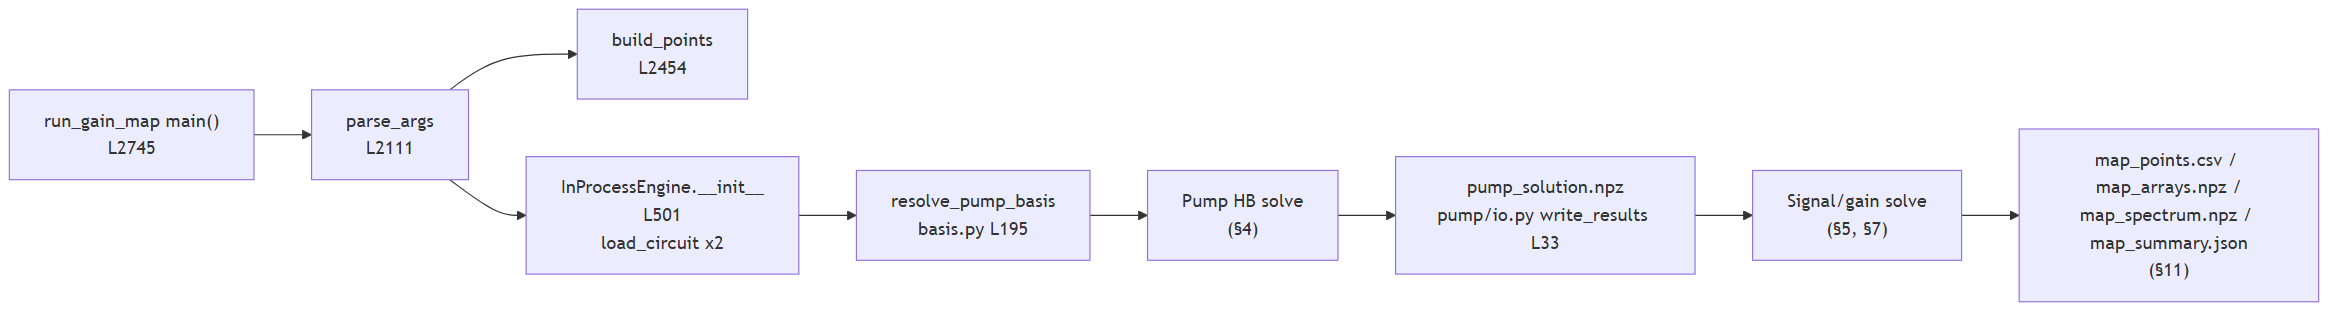
\includegraphics[width=1\linewidth,height=\textheight,keepaspectratio]{diagrams_png/diag_000.png}

\begin{center}\rule{0.5\linewidth}{0.5pt}\end{center}

\section{4. Pump solver}\label{pump-solver}

\subsection{4.1 Top-level pump execution
flow}\label{top-level-pump-execution-flow}

\begin{verbatim}
CLI (run_gain_map)                       src file / function / lines
  parse_args                             run_gain_map.py parse_args 2111-2451
  → build_points (dBm→peak current)      run_gain_map.py build_points 2454; dbm_to_peak_current_a 76
  → executor dispatch                    run_gain_map.py main 2774-2830
      inprocess → InProcessEngine        run_gain_map.py InProcessEngine 490
      subprocess → run_point→EXP08       run_gain_map.py run_point 298 (experiments/exp08_*)
  → traversal dispatch                   run_gain_map.py main 2818-2824
      column      → run_warm_pass_inprocess   1195
      non-column  → run_map_traversal         1717
  → per cell: engine.solve_point         run_gain_map.py solve_point 606
      build problem                      _build_problem 546 → FullIPMPumpProblem (problem.py 89)
      Schur reduce (optional)            _make_solve_problem 561 → build_schur_problem (schur_operators.py 300)
      solve                              HarmonicNewtonKrylovSolver (solver.py 127)
      write pump                         summarize_solution/write_results (pump/io.py 13/33)
  → gain solve (if converged/force)      _gain 980 (§7)
  → status/gate/serialize               evaluate_gate 1835; write_* 1904-2109; main 2842-2893
\end{verbatim}

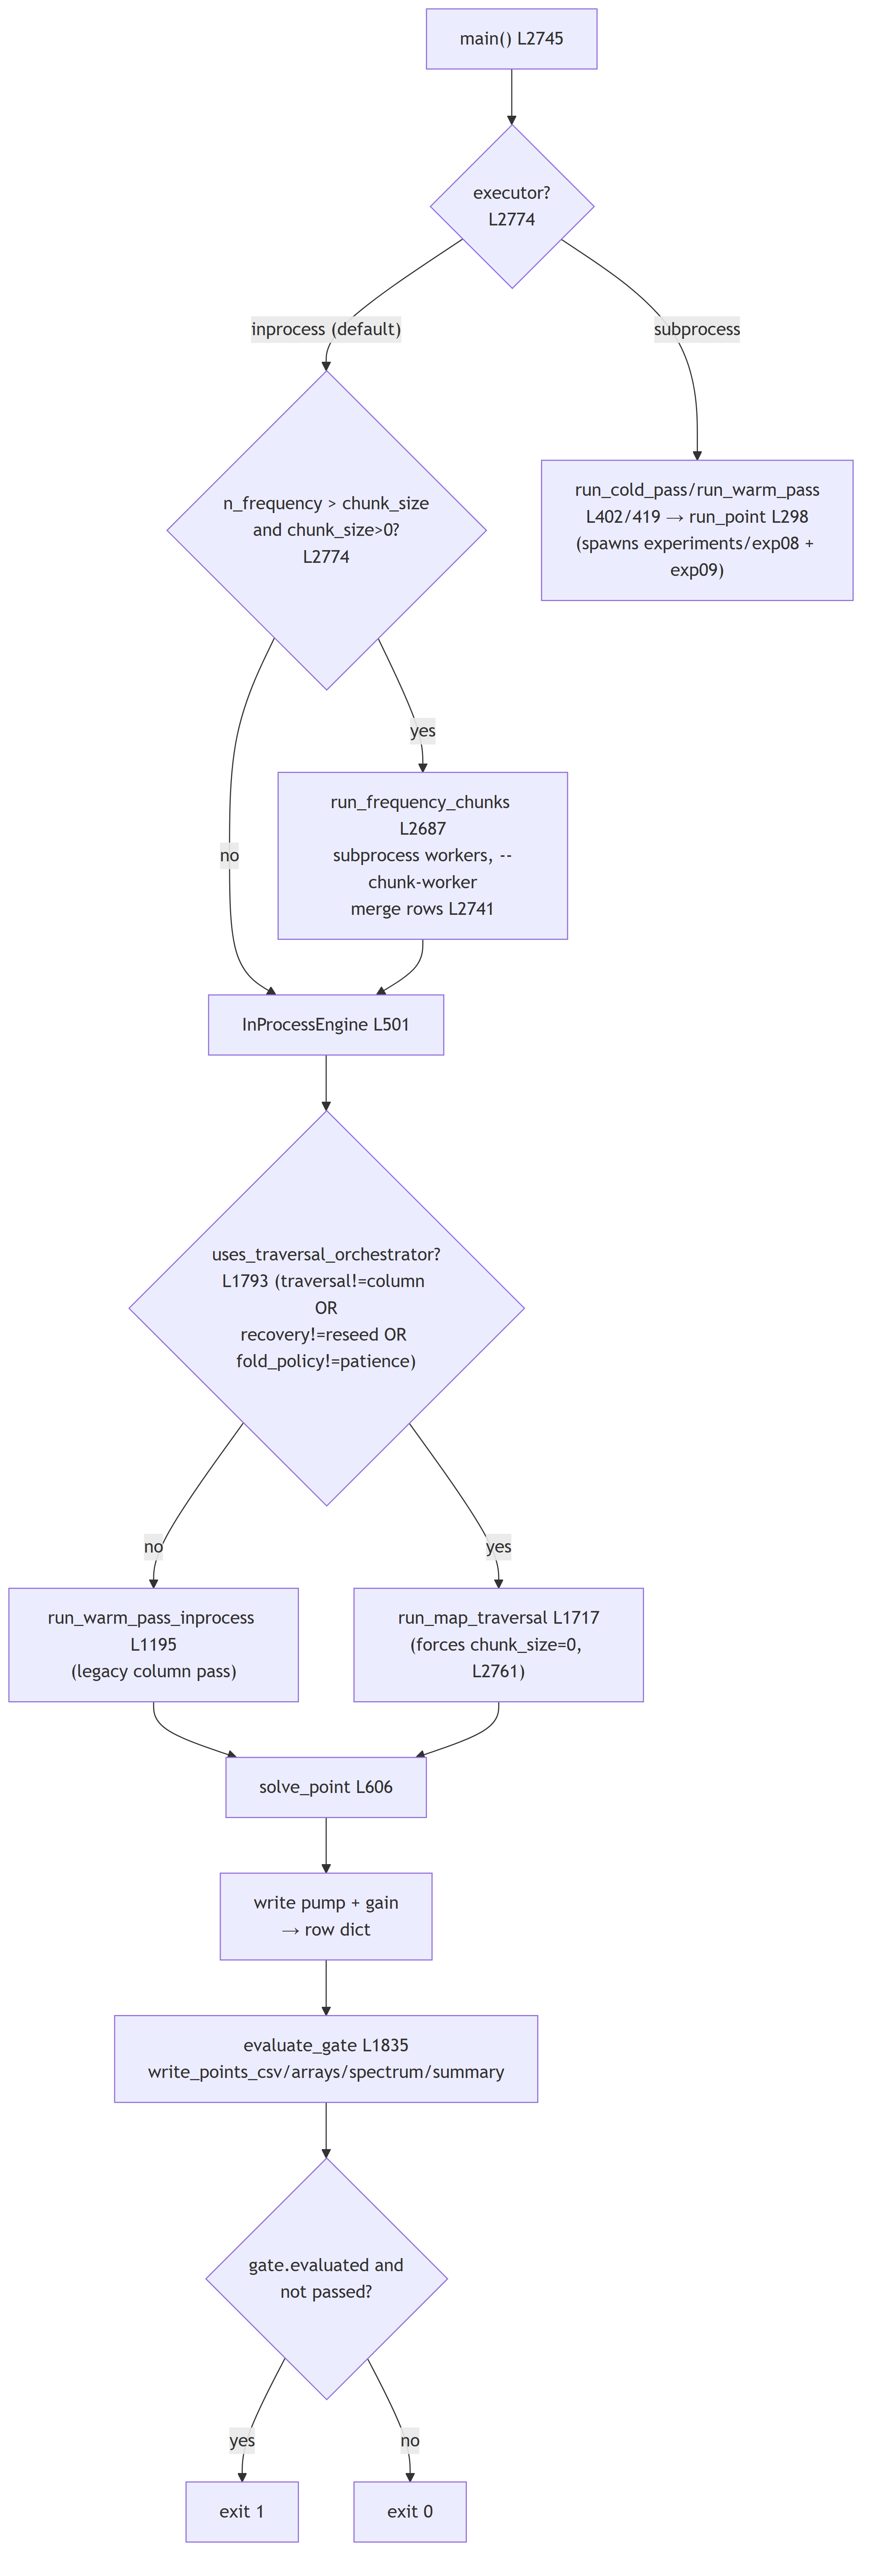
\includegraphics[width=1\linewidth,height=\textheight,keepaspectratio]{diagrams_png/diag_001.png}

\subsection{4.2 Pump problem assembly}\label{pump-problem-assembly}

\texttt{InProcessEngine.\_build\_problem} (L546) constructs a
\texttt{FullIPMPumpProblem} (alias of \texttt{FullPumpProblem},
\texttt{problem.py} L89, alias L423). Key state:

\begin{itemize}
\tightlist
\item
  \textbf{Unknown representation:} complex array \texttt{X} of shape
  \texttt{(H,\ n)} = (\texttt{n\_modes}, \texttt{n\_nodes}),
  \texttt{problem.zeros()} (L145). Packed to real via
  \texttt{pack\_complex} (\texttt{{[}Re…;\ Im…{]}}, L67) for GMRES.
\item
  \textbf{Per-mode linear blocks}
  \texttt{D\_k\ =\ K\ -\ (kω)²C\ +\ i(kω)G}, built once
  (\texttt{\_build\_linear\_blocks} L132) as complex CSC.
\item
  \textbf{Source} \texttt{source\_coeffs(λ)} (L148): only row
  \texttt{source\_row} (the fundamental mode), node
  \texttt{pump\_node\_index}, value \texttt{0.5·λ·pump\_current\_a}.
  \texttt{λ} (\texttt{source\_scale}) is the natural continuation
  parameter (linear in the source).
\item
  \textbf{Residual} \texttt{residual\_coeffs(X,\ λ)} (L177):
  \texttt{D\_k\ X\_k\ +\ N\_k(X)\ −\ S\_k}, where \texttt{N} is the
  projected Josephson current (\texttt{nonlinear\_current\_coeffs} L174
  via time-domain synth \texttt{grid.synthesize} \texttt{2·Re(E·X)},
  L41).
\item
  \textbf{JVP} (matrix-free tangent apply)
  \texttt{jvp\_coeffs\_with\_tangent} (L195): analytic AFT
  Jacobian-vector product
  \texttt{D\_k\ V\_k\ +\ AFT{[}γ(t)·(Bphiᵀ\ v(t)){]}}. \textbf{Not}
  finite-difference, not autodiff (\texttt{backends/jvp\_backends.py}
  documents this; \texttt{fd\_jvp} exists only for tests).
\end{itemize}

\textbf{What the solver actually assembles.} In the harmonic
(frequency-domain) basis the pump residual for mode \(k\), the per-mode
linear operator, and the matrix-free tangent apply are

\[
R_k(X,\lambda) = D_k X_k + N_k(X) - S_k(\lambda),
\qquad
D_k = K - (k\omega_p)^2 C + i\,(k\omega_p)\,G,
\]

\[
S_k(\lambda) = \tfrac{1}{2}\,\lambda\, I_{\mathrm{pump}}\,\delta_{k,1}\ \text{at the pump node},
\qquad
N_k(X) = \mathcal{F}_k\!\Big[B_\phi\, I_c \sin\!\big(B_\phi^{\top} x(t)/\phi_0\big)\Big],
\]

where \(x(t)=2\,\mathrm{Re}\sum_{k} X_k e^{ik\omega_p t}\) is the real
waveform in the JC positive-phasor convention and \(\mathcal{F}_k\) is
the alias-free Fourier projection onto mode \(k\). Rather than form the
Jacobian \(J=\partial R/\partial X\), the solver applies it to a vector
\(V\) directly (this is what GMRES needs):

\[
\big(J\,V\big)_k = D_k V_k + \mathcal{F}_k\!\Big[\gamma(t)\,\big(B_\phi^{\top} v(t)\big)\Big],
\qquad \gamma(t)=\cos\!\big(\psi_p(t)/\phi_0\big)\,\tfrac{I_c}{\phi_0},
\]

i.e.~the linear block plus the parametric coupling \(\gamma(t)\)
evaluated at the current pump iterate. This same \(\gamma(t)\) is what
the signal solve later reuses (§9).

\subsection{\texorpdfstring{4.3 Pump backend dispatch
(\texttt{-\/-inproc-pump-backend})}{4.3 Pump backend dispatch (-\/-inproc-pump-backend)}}\label{pump-backend-dispatch---inproc-pump-backend}

Two accepted values (\texttt{parse\_args} L2225):

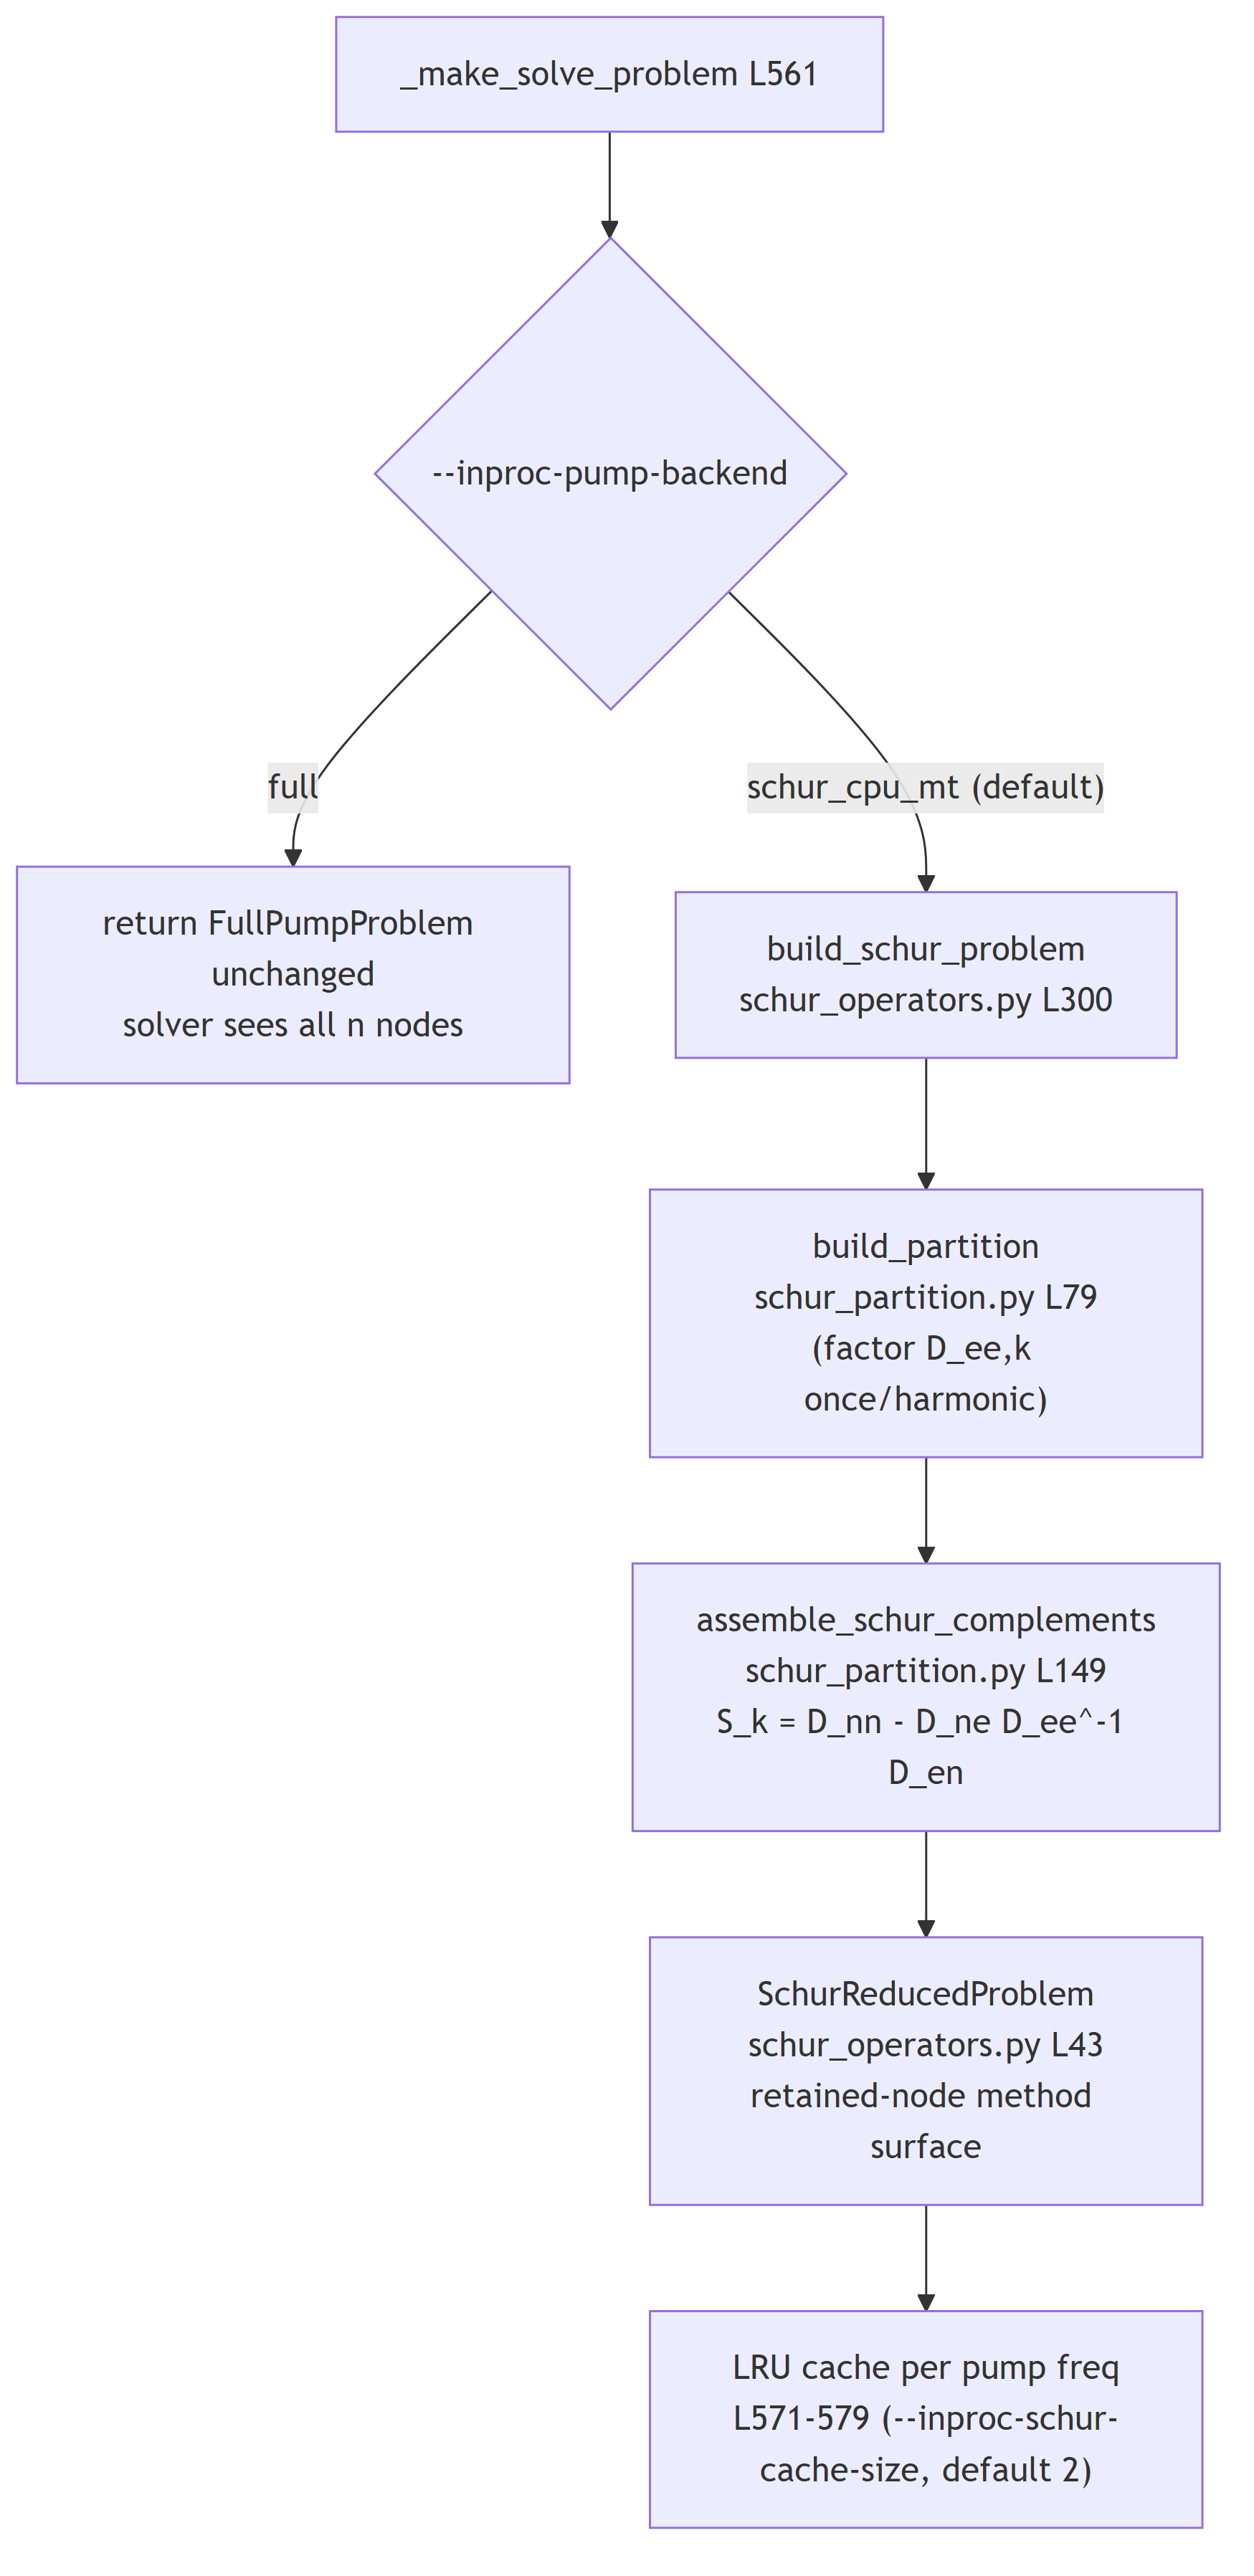
\includegraphics[width=1\linewidth,height=\textheight,keepaspectratio]{diagrams_png/diag_002.png}

{\def\LTcaptype{none} % do not increment counter
\begin{longtable}[]{@{}
  >{\raggedright\arraybackslash}p{(\linewidth - 4\tabcolsep) * \real{0.3333}}
  >{\raggedright\arraybackslash}p{(\linewidth - 4\tabcolsep) * \real{0.3333}}
  >{\raggedright\arraybackslash}p{(\linewidth - 4\tabcolsep) * \real{0.3333}}@{}}
\toprule\noalign{}
\begin{minipage}[b]{\linewidth}\raggedright
Aspect
\end{minipage} & \begin{minipage}[b]{\linewidth}\raggedright
\texttt{full}
\end{minipage} & \begin{minipage}[b]{\linewidth}\raggedright
\texttt{schur\_cpu\_mt} (default)
\end{minipage} \\
\midrule\noalign{}
\endhead
\bottomrule\noalign{}
\endlastfoot
Unknown & complex \texttt{(H,\ n)} all nodes & complex \texttt{(H,\ m)}
retained nodes (\texttt{SchurReducedProblem.zeros} L103) \\
Residual & \texttt{FullPumpProblem.residual\_coeffs} L177 &
\texttt{SchurReducedProblem.residual\_coeffs} L124 (uses \texttt{S\_k}
apply, retained \texttt{Bphi\_r}) \\
Linear apply & dense per-block \texttt{D\_k} matvec & \texttt{S\_k}
assembled matvec (\texttt{\_lin\_apply} L96, mode \texttt{assembled}) or
matrix-free \texttt{reduced\_linear\_apply}
(\texttt{schur\_partition.py} L203) \\
JVP & \texttt{jvp\_coeffs\_with\_tangent} L195 &
\texttt{jvp\_coeffs\_with\_tangent} L138 (retained) \\
Post-solve & \texttt{X} is full already & \texttt{reconstruct\_full}
(\texttt{back\_substitute\_full} L217) once after convergence for
exp09 \\
Factorization reuse & none of \texttt{D\_ee} & \texttt{D\_ee,k} factored
once per frequency (constant in X), reused every Newton/Krylov iter \\
Device & CPU (scipy SuperLU / MKL PARDISO) & CPU (same) \\
\end{longtable}
}

\texttt{build\_schur\_problem} retains \textbf{Josephson-incident nodes
plus requested ports} (\texttt{engine.ports}, L510;
\texttt{build\_partition} L106). The \texttt{linear\_apply\_mode} and
harmonic-band cutoffs (\texttt{precond\_ell\_diff\_max/sum\_max}) are
constructor knobs of \texttt{SchurReducedProblem} (schur\_operators.py
L60--68) but are \textbf{not exposed on the CLI} --- always defaults
(\texttt{assembled}, no banding). Cache is an insertion-ordered dict
acting as an LRU (\texttt{\_schur\_part\_cache} L517, evict-oldest
L577).

\textbf{The reduction.} Per harmonic the nodes are split into
\emph{retained} \(n\) (Josephson-incident nodes plus requested ports)
and \emph{eliminated} \(e\). Factoring the constant block \(D_{ee,k}\)
once per pump frequency yields the Schur complement and the reduced
residual solved on the retained nodes only:

\[
S_k = D_{nn,k} - D_{ne,k}\,D_{ee,k}^{-1} D_{en,k},
\qquad
R^{\mathrm{red}}_k = S_k\,X_k^{(n)} + N_k^{(n)}(X) - S^{\mathrm{src}}_k .
\]

The eliminated part is recovered by one back-substitution
\(x_e = D_{ee}^{-1}\!\big(s_e - D_{en}\,x_n\big)\) after convergence
(for the exp09 hand-off). Because \(D_{ee,k}\) does not depend on \(X\),
its factorization is reused across every Newton and Krylov iteration ---
the main reason the Schur backend is the default.

\textbf{Warm-start / cold-start selection} happens in
\texttt{solve\_point} (L640):

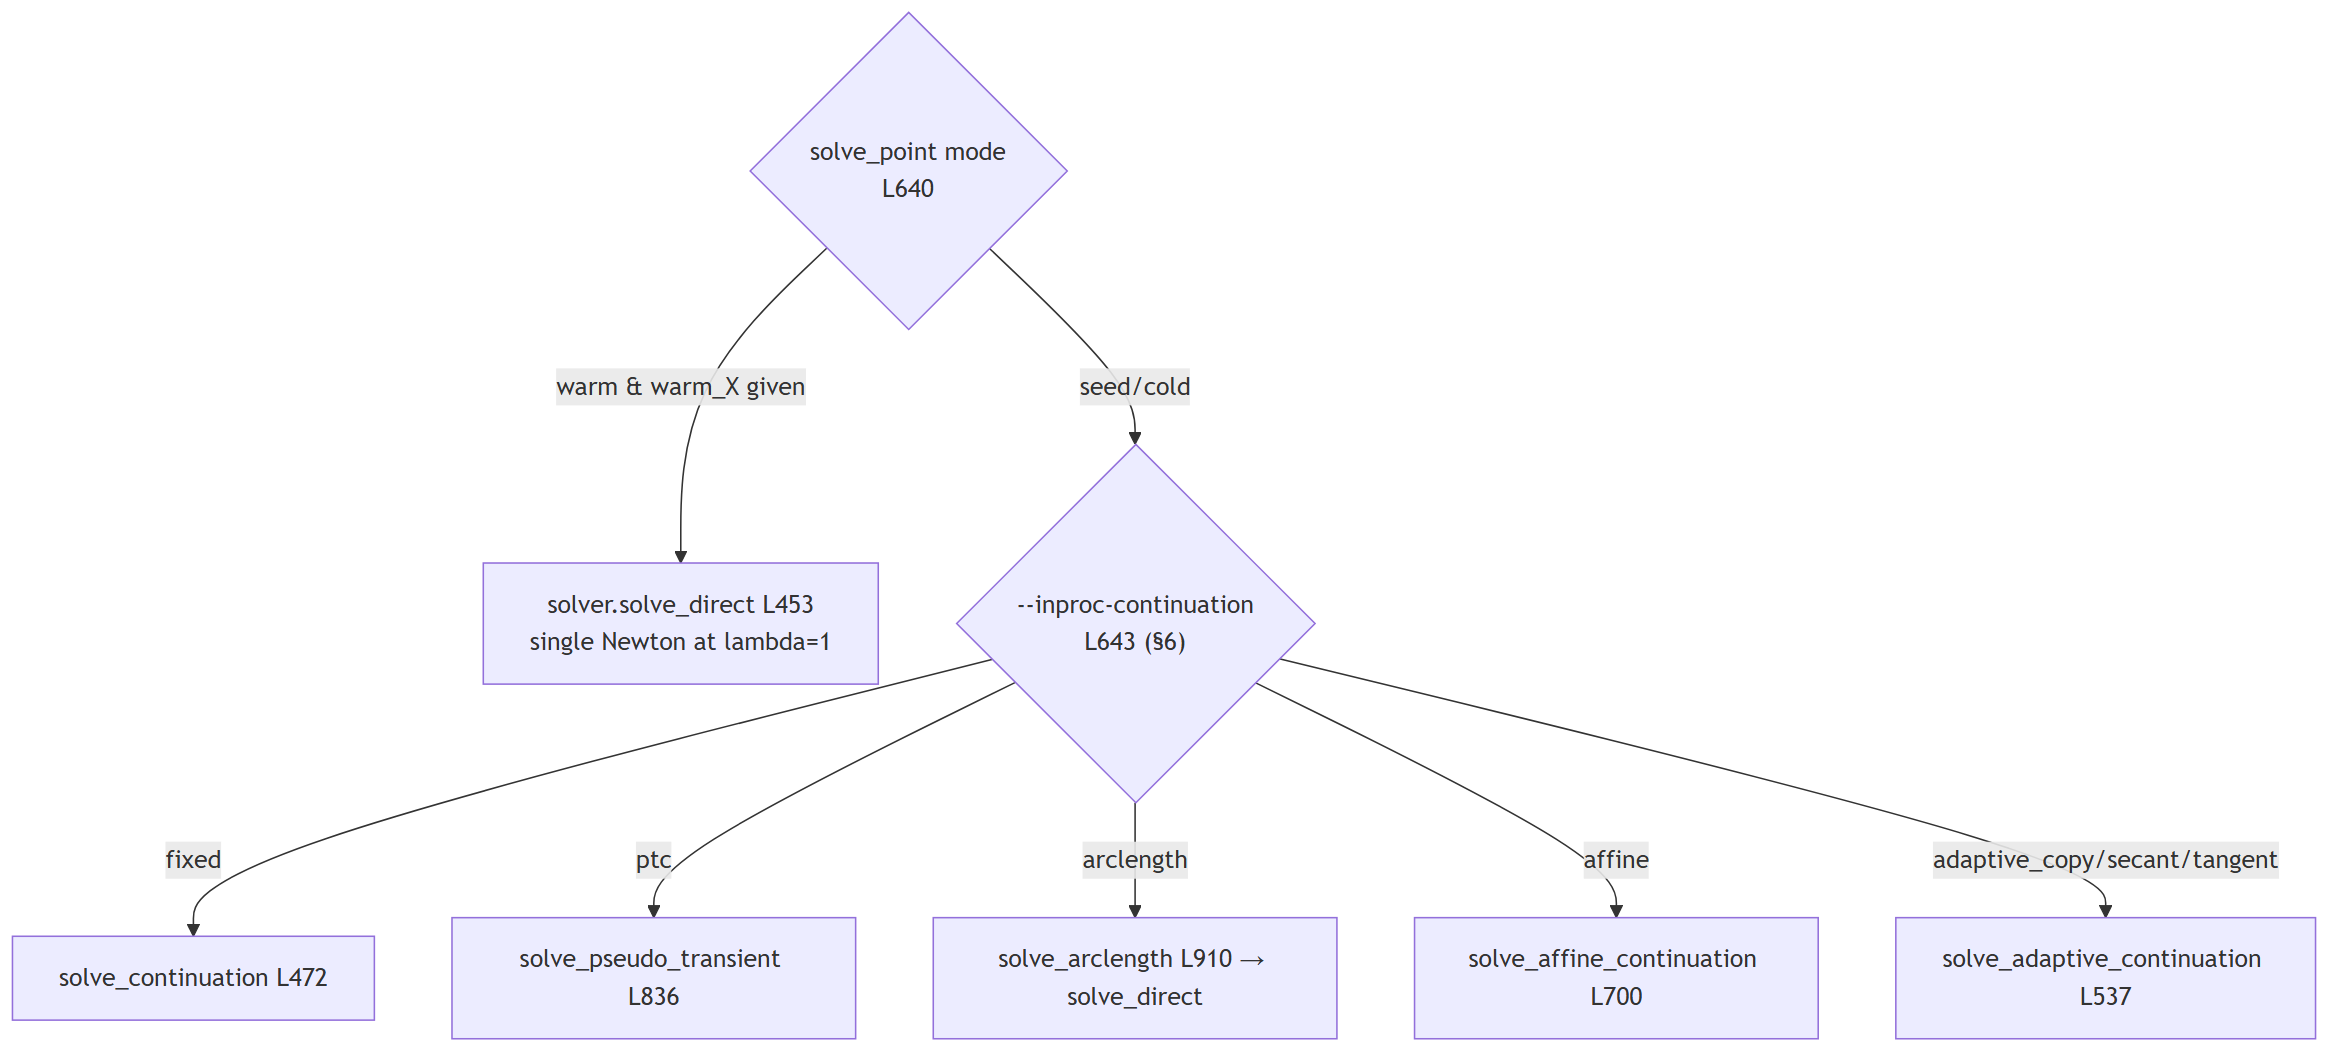
\includegraphics[width=1\linewidth,height=\textheight,keepaspectratio]{diagrams_png/diag_003.png}

\subsection{4.4 Convergence acceptance and
status}\label{convergence-acceptance-and-status}

\texttt{converged} is set in \texttt{solve\_point} L724 as
\texttt{reports{[}-1{]}.converged\ and\ \textbar{}source\_scale\ −\ 1.0\textbar{}\ \textless{}\ 1e-12}
--- i.e.~the last solve must have converged \textbf{at full drive λ=1}.
A converged-at-λ\textless1 continuation that stalls short of full drive
is \textbf{not} counted as converged. Row \texttt{pump\_status} becomes
\texttt{VALID\_CONVERGED} else \texttt{FAIL} (L748).

\begin{center}\rule{0.5\linewidth}{0.5pt}\end{center}

\section{5. Signal solver}\label{signal-solver}

\subsection{\texorpdfstring{5.1 Signal backend dispatch
(\texttt{-\/-signal-backend},
\texttt{-\/-signal-solver})}{5.1 Signal backend dispatch (-\/-signal-backend, -\/-signal-solver)}}\label{signal-backend-dispatch---signal-backend---signal-solver}

\texttt{InProcessEngine.\_solve\_signal} (L1059) selects the linear
backend; \texttt{solve\_linear\_system} (\texttt{floquet.py} L199)
selects the sparse solver.

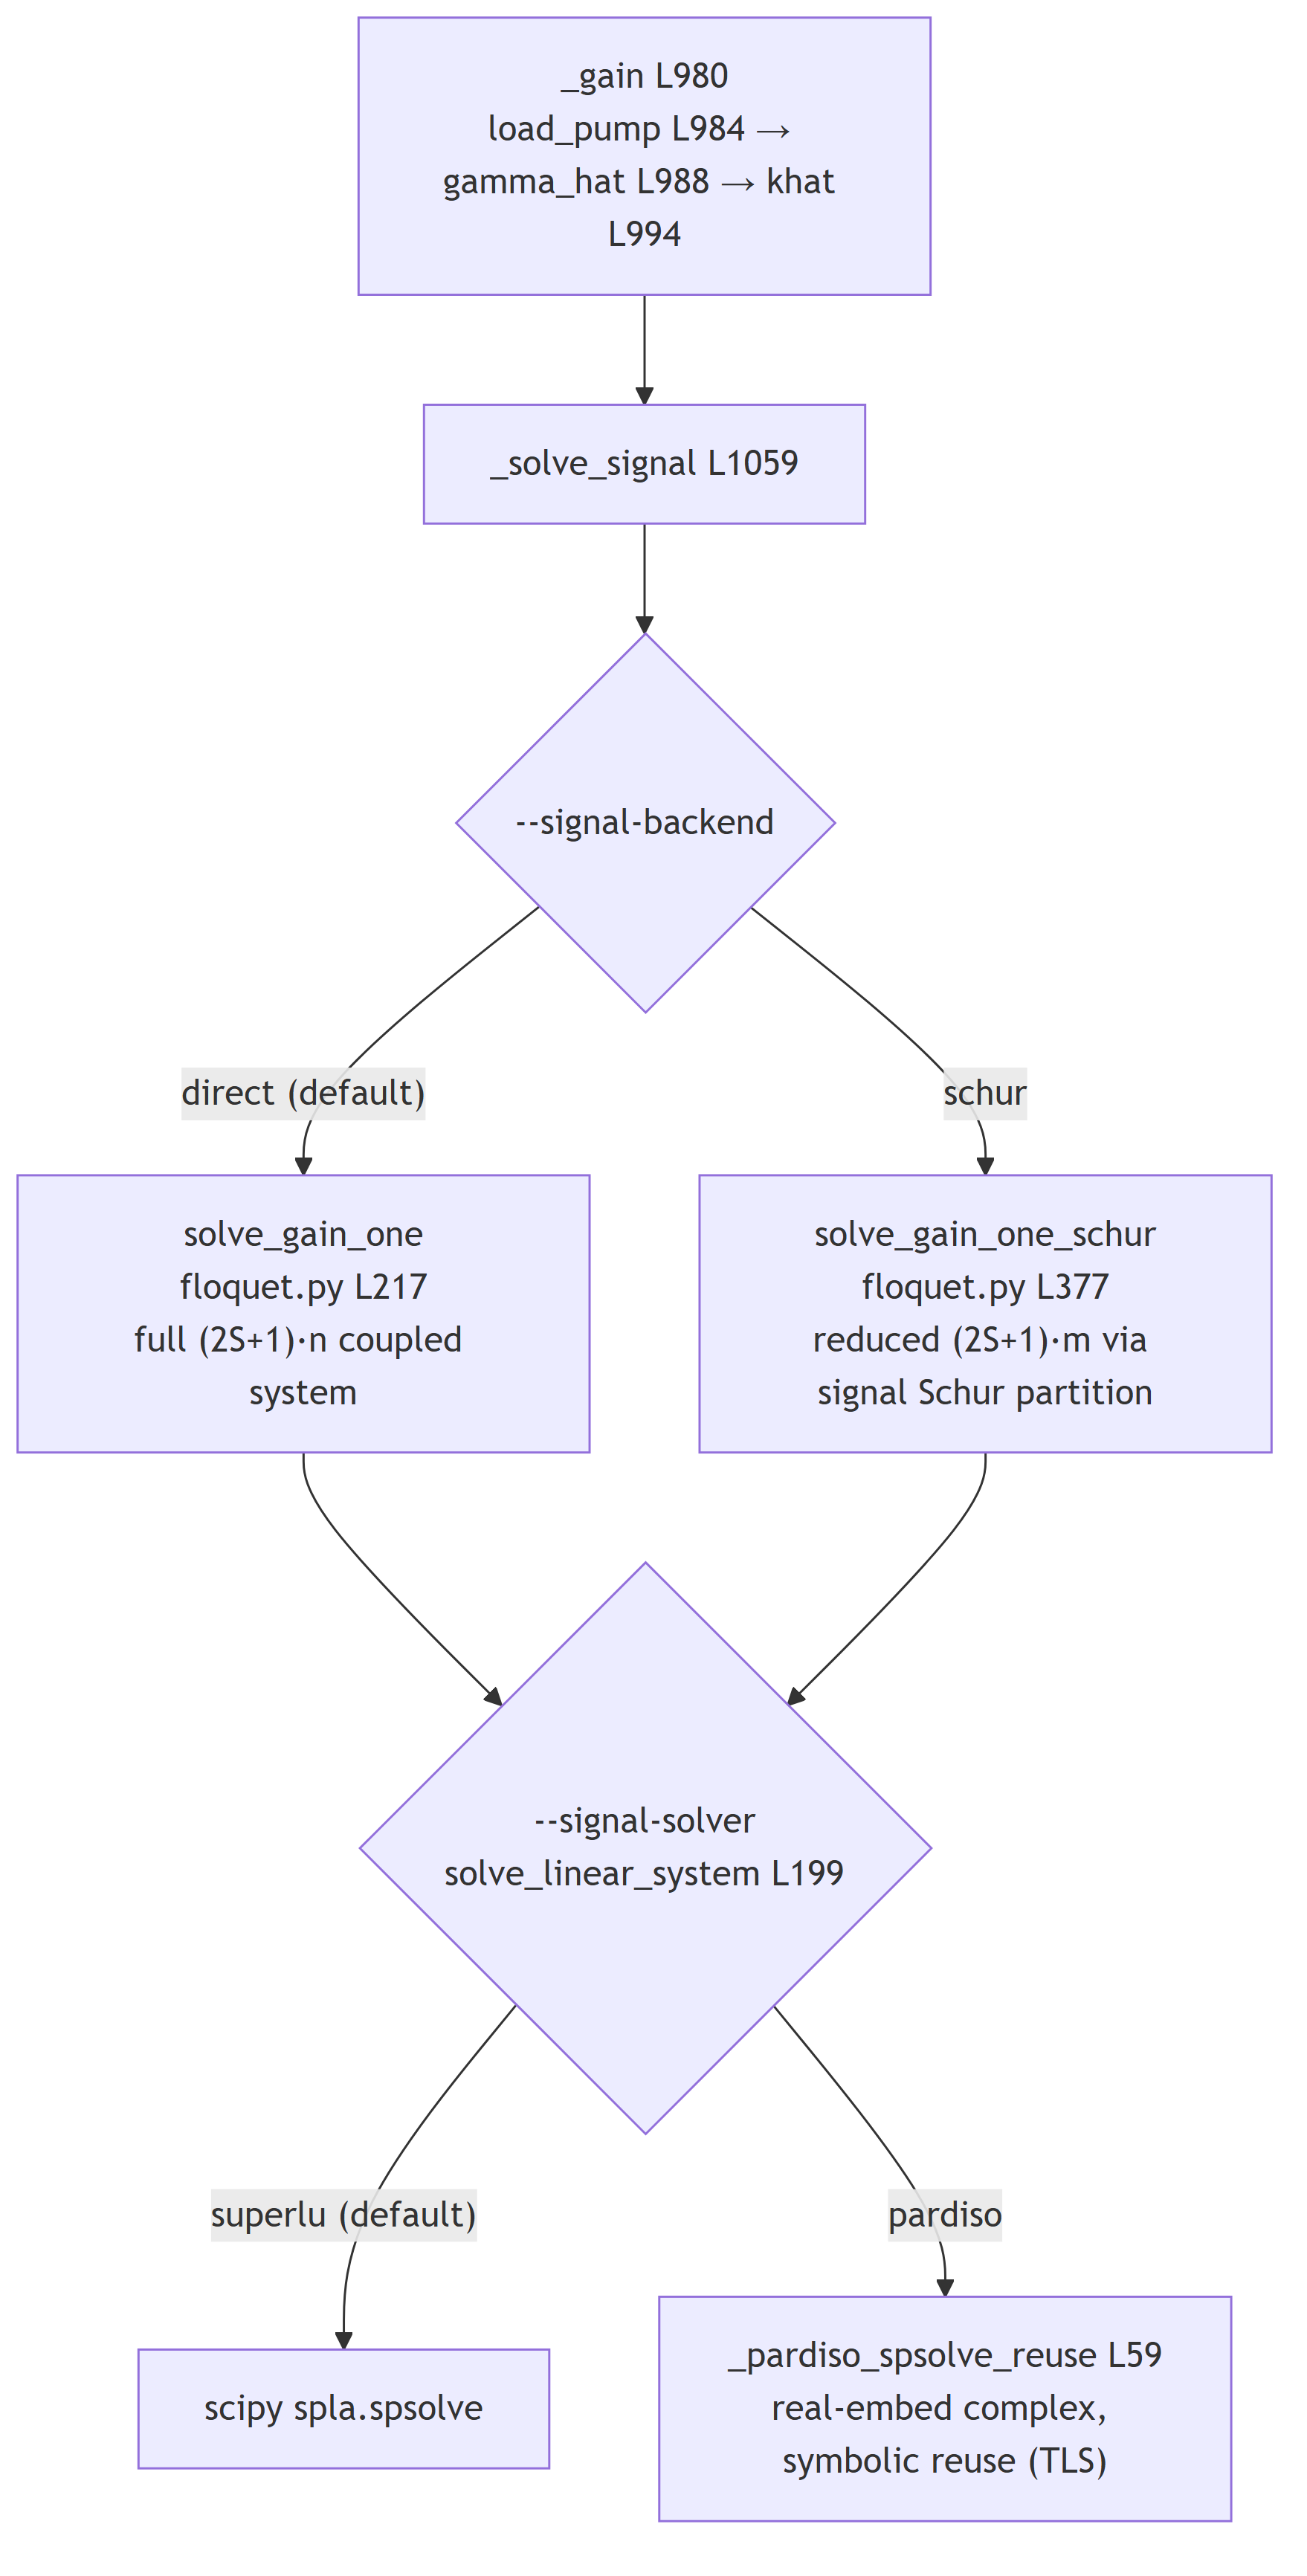
\includegraphics[width=1\linewidth,height=\textheight,keepaspectratio]{diagrams_png/diag_004.png}

{\def\LTcaptype{none} % do not increment counter
\begin{longtable}[]{@{}
  >{\raggedright\arraybackslash}p{(\linewidth - 4\tabcolsep) * \real{0.3333}}
  >{\raggedright\arraybackslash}p{(\linewidth - 4\tabcolsep) * \real{0.3333}}
  >{\raggedright\arraybackslash}p{(\linewidth - 4\tabcolsep) * \real{0.3333}}@{}}
\toprule\noalign{}
\begin{minipage}[b]{\linewidth}\raggedright
Aspect
\end{minipage} & \begin{minipage}[b]{\linewidth}\raggedright
\texttt{direct} (\texttt{solve\_gain\_one} L217)
\end{minipage} & \begin{minipage}[b]{\linewidth}\raggedright
\texttt{schur} (\texttt{solve\_gain\_one\_schur} L377)
\end{minipage} \\
\midrule\noalign{}
\endhead
\bottomrule\noalign{}
\endlastfoot
Sideband set & \texttt{sideband\_list(S)} = \texttt{{[}-S..S{]}},
\texttt{2S+1} blocks (L84) & same \\
Sideband ordering/index & block \texttt{m} at rows
\texttt{ms.index(m)·n}; RHS at \texttt{signal\_m=0} (L149/L1084) & same
but block stride \texttt{m\_red} (retained) \\
System assembly &
\texttt{assemble\_conversion\_matrix{[}\_from\_base{]}} L115/L103:
block(m,q)=\texttt{khat{[}m−q{]}} + \texttt{D(ω\_s+mω\_p)} on diag &
reduced blocks \texttt{khat\_n{[}m−q{]}} + \texttt{part.schur{[}m{]}}
(L414) \\
Formulation & full node system, \textbf{complex} & Schur-reduced
retained system, complex; \texttt{build\_signal\_schur\_partition}
L359 \\
Solve & direct sparse factor-solve (\texttt{solve\_linear\_system}) &
same, smaller matrix \\
Factor reuse & none across signal freqs (each \texttt{A} differs);
\texttt{khat\_big\_base} reused across spectrum points (L1010) & signal
Schur \textbf{partition} cached per (ω\_p, ω\_s, S, ports) key
(L1063--1080), \texttt{-\/-inproc-schur-cache-size} bound \\
Baselines & always: off (\texttt{khat\_off\_0}) + pump-diagonal
(\texttt{khat{[}0{]}}) via \texttt{solve\_single\_block\_transfer} L176
& optional --- skipped if \texttt{-\/-skip-baselines} (L447),
\texttt{gain\_db} still valid \\
Gain extraction & \texttt{vout\_on\ =\ iω\_s·φ\_out}; S-param
\texttt{port\_s\_from\_unit\_current\_response} L69;
\texttt{gain\_db\ =\ 20·log10\textbar{}S\textbar{}}
(\texttt{gain\_db\_from\_s} L16) & same, retained positions
\texttt{part.retained\_pos} \\
Failure / nonfinite & \texttt{status="CHECK"} if
\texttt{¬isfinite(gain)} or
\texttt{linear\_rel\_residual\ \textgreater{}\ 1e-7} (L318) &
\texttt{status="CHECK"} if \texttt{¬isfinite(\textbar{}S\textbar{})} or
resid\textgreater1e-7 (L487) \\
\end{longtable}
}

\texttt{gain\_status} becomes \texttt{VALID\_SOLVED} only when
\texttt{GainResult.status\ ==\ "VALID\_SOLVED"} (solve\_point L797). Any
\texttt{CHECK} (nonfinite or high residual) leaves the row
\texttt{gain\_db} populated but the cell status \texttt{ERROR}
(solve\_point L805).

\subsection{5.2 Signal frequency
construction}\label{signal-frequency-construction}

\begin{itemize}
\tightlist
\item
  Trailing (map) signal: \texttt{signal\_ghz\_for} (L109) =
  \texttt{-\/-signal-ghz} if set, else
  \texttt{pump\_ghz\ −\ -\/-signal-detuning-mhz/1000} (tracks pump).
\item
  Spectrum ladder (\texttt{-\/-signal-spectrum}, default on):
  \texttt{spectrum\_offsets\_mhz} (L121) builds ±offsets
  \texttt{start,\ start+step,\ …} (\texttt{-\/-signal-offset-*}), solved
  in \texttt{\_gain} L1016--1039.
\end{itemize}

\subsection{5.3 Parallel workers}\label{parallel-workers}

\texttt{-\/-signal-workers} (default 6) → a \texttt{ThreadPoolExecutor}
over spectrum signal points (\texttt{\_gain} L1025--1027). Threads share
the read-only \texttt{khat}, \texttt{khat\_off\_0},
\texttt{khat\_big\_base}. PARDISO calls are guarded per-thread
(\texttt{\_PARDISO\_TLS} L46, \texttt{\_pardiso\_thread\_context} L26
limiting BLAS threads via \texttt{TWPA\_PARDISO\_THREADS}). \texttt{1} =
serial.

\begin{center}\rule{0.5\linewidth}{0.5pt}\end{center}

\section{6. Continuation controller}\label{continuation-controller}

Two distinct continuation layers exist:

\begin{itemize}
\tightlist
\item
  \textbf{Intra-cell} (in pump amplitude λ, one cell):
  \texttt{-\/-inproc-continuation} → \texttt{solver.py}.
\item
  \textbf{Inter-cell} (across pump power and, in traversal mode,
  frequency): the warm-pass / traversal orchestration in
  \texttt{run\_gain\_map.py}, plus the recovery ladders.
\end{itemize}

\subsection{\texorpdfstring{6.1 Intra-cell
(\texttt{-\/-inproc-continuation}, 7
values)}{6.1 Intra-cell (-\/-inproc-continuation, 7 values)}}\label{intra-cell---inproc-continuation-7-values}

Dispatched in \texttt{solve\_point} L643--720. Every value is
implemented (none unsupported).

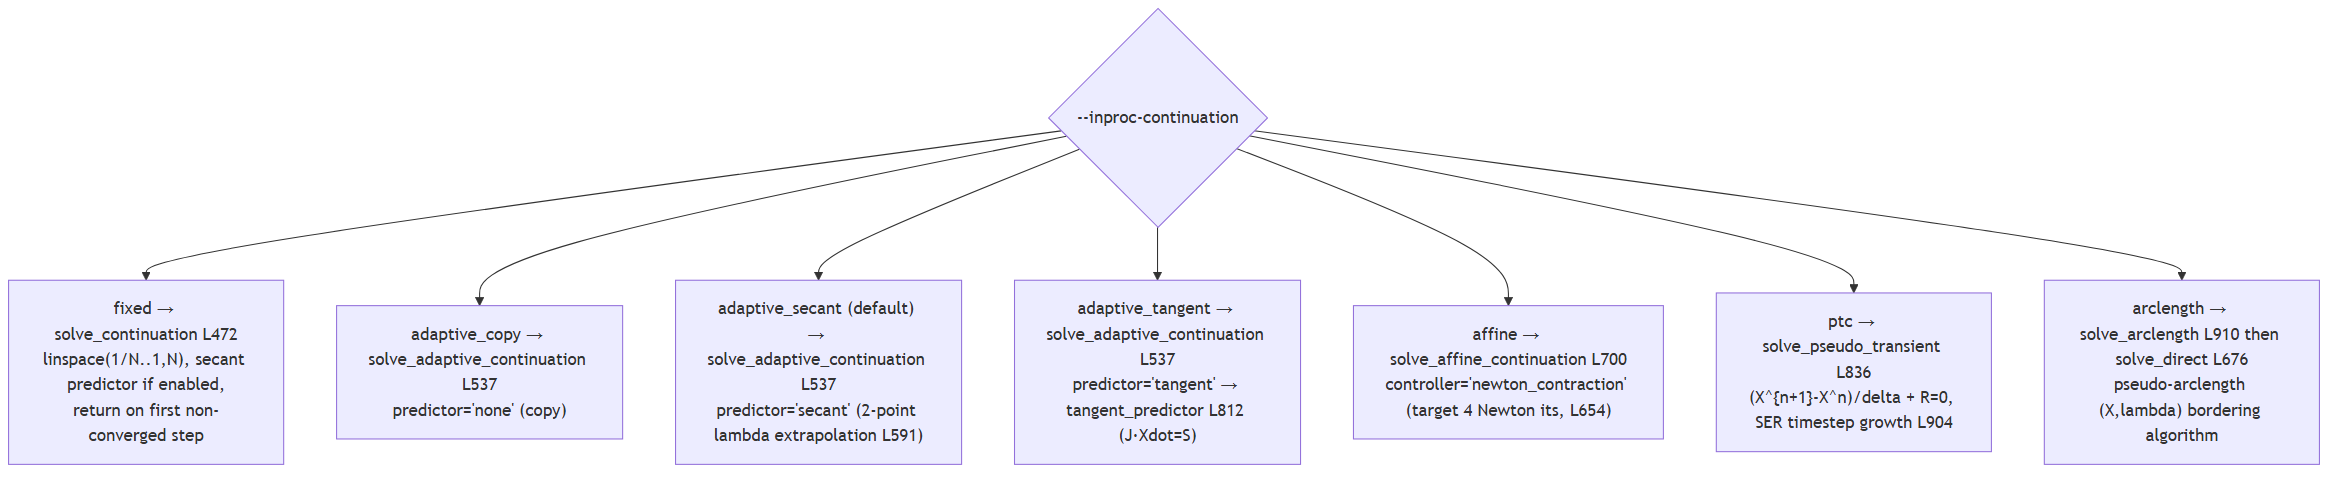
\includegraphics[width=1\linewidth,height=\textheight,keepaspectratio]{diagrams_png/diag_005.png}

Adaptive step controller (\texttt{solve\_adaptive\_continuation} L537):

\begin{itemize}
\tightlist
\item
  Seed \texttt{X} = \texttt{x\_init} or zeros; \texttt{λ=0},
  \texttt{step=-\/-adaptive-initial-step} (default 1.0).
\item
  Predictor per value; a \textbf{predictor guard} (L601--623) rejects
  any predicted guess whose residual is
  \texttt{\textgreater{}max(100·copy\_residual,\ 1e6)} or non-finite →
  falls back to copy.
\item
  On converge: \texttt{λ←target},
  \texttt{step←min(1,\ max(min\_step,\ step·growth))} with
  \texttt{growth=1.5} (or the affine \texttt{newton\_contraction} rule
  L654--659). Loop until \texttt{λ\ ≥\ 1−1e-12}.
\item
  On fail: \texttt{step←step·shrink} (\texttt{shrink=0.5}); if
  \texttt{step\textless{}min\_step} (\texttt{-\/-adaptive-min-step}
  default 0.05) → \textbf{fixed fallback}
  \texttt{solve\_continuation(fallback\_fixed\_steps)}
  (\texttt{-\/-inproc-fallback-fixed-steps} default 20) L682,
  \texttt{trace.fallback\_used=True}.
\item
  \textbf{Deadline:} \texttt{max\_wall\_s} =
  \texttt{-\/-inproc-continuation-deadline-s} if \textgreater0 else
  \texttt{-\/-inproc-solve-deadline-s} (solve\_point L686--690). Checked
  at loop top (L573) and before fallback (L670).
\end{itemize}

Fixed (\texttt{solve\_continuation} L472): \texttt{λ} over
\texttt{linspace(1/N,\ 1,\ N)} (\texttt{-\/-continuation-steps} default
20), optional secant predictor (L496), returns immediately on the first
non-converged \texttt{λ} (L527).

\textbf{The math of a predictor step.} All intra-cell methods drive the
drive parameter \(\lambda:0\to1\) solving \(R(X,\lambda)=0\), differing
only in how they predict the next Newton guess. With
\(S=\partial R/\partial\lambda\) the source sensitivity:

\[
\text{secant:}\quad X^{\mathrm{p}} = X_j + \frac{\lambda^\star-\lambda_j}{\lambda_j-\lambda_{j-1}}\,(X_j - X_{j-1}),
\qquad
\text{tangent:}\quad J\,\dot X = S,\ \ X^{\mathrm{p}} = X_j + \Delta\lambda\,\dot X .
\]

Pseudo-transient continuation (PTC) instead damps toward the root with a
pseudo-timestep \(\delta\) grown by the switched-evolution-relaxation
(SER) rule:

\[
\frac{X^{n+1}-X^{n}}{\delta} + R(X^{n+1}) = 0,
\qquad
\delta \leftarrow \delta\,\frac{\lVert R^{n-1}\rVert}{\lVert R^{n}\rVert}.
\]

Pseudo-arclength replaces \(\lambda\) by arclength \(s\) as the marching
variable and appends a tangent-plane constraint, which lets it round a
\textbf{fold} (turning point) where \(\dot\lambda\) changes sign --- a
place natural-parameter continuation cannot pass:

\[
R(X,\lambda)=0,\qquad
\dot X^{\top}(X-X_0) + \dot\lambda\,(\lambda-\lambda_0) - \Delta s = 0 .
\]

PTC (\texttt{solve\_pseudo\_transient} L836): modified-Newton with shift
\texttt{1/δ} via \texttt{\_solve\_linear} (shift arg L881); damped
acceptance on true residual (L892); SER growth
\texttt{δ←max(δ,\ δ·prev/curr)} (L904);
\texttt{max\_it\ =\ 4·max\_newton}; deadline honored (L861, L884).

Pseudo-arclength (\texttt{solve\_arclength} L910): joint
\texttt{(X,\ λ)}, tangent-plane constraint; bordering algorithm --- one
predictor-point factorization reused across corrector iterations
(\texttt{\_linear\_solver} L736), two solves \texttt{J\ a=−R},
\texttt{J\ b=S} per corrector (L973/L981); fold detected as sign change
of \texttt{λ\_dot} (L1010); target crossing interpolated (L1013).
Returns \texttt{(X,\ λ,\ info)} with \texttt{reached\_target},
\texttt{fold\_lambda}, \texttt{terminal\_reason} ∈
\texttt{\{target,\ deadline,\ minimum\_step,\ max\_steps\}}.

\subsection{6.2 Inter-cell continuation (power axis --- legacy column
pass)}\label{inter-cell-continuation-power-axis-legacy-column-pass}

\texttt{run\_warm\_pass\_inprocess} (L1195): per frequency column,
ascending power. Each cell warm- starts from the previous converged pump
\texttt{X} via \texttt{solve\_direct} (single full-scale Newton).
Predictor \texttt{-\/-inproc-fold-predictor}
(\texttt{none}\textbar{}\texttt{secant}, default \texttt{secant}) builds
the guess by \texttt{secant\_guess} (L1111) extrapolating along the
pump-current axis from the last two converged states.

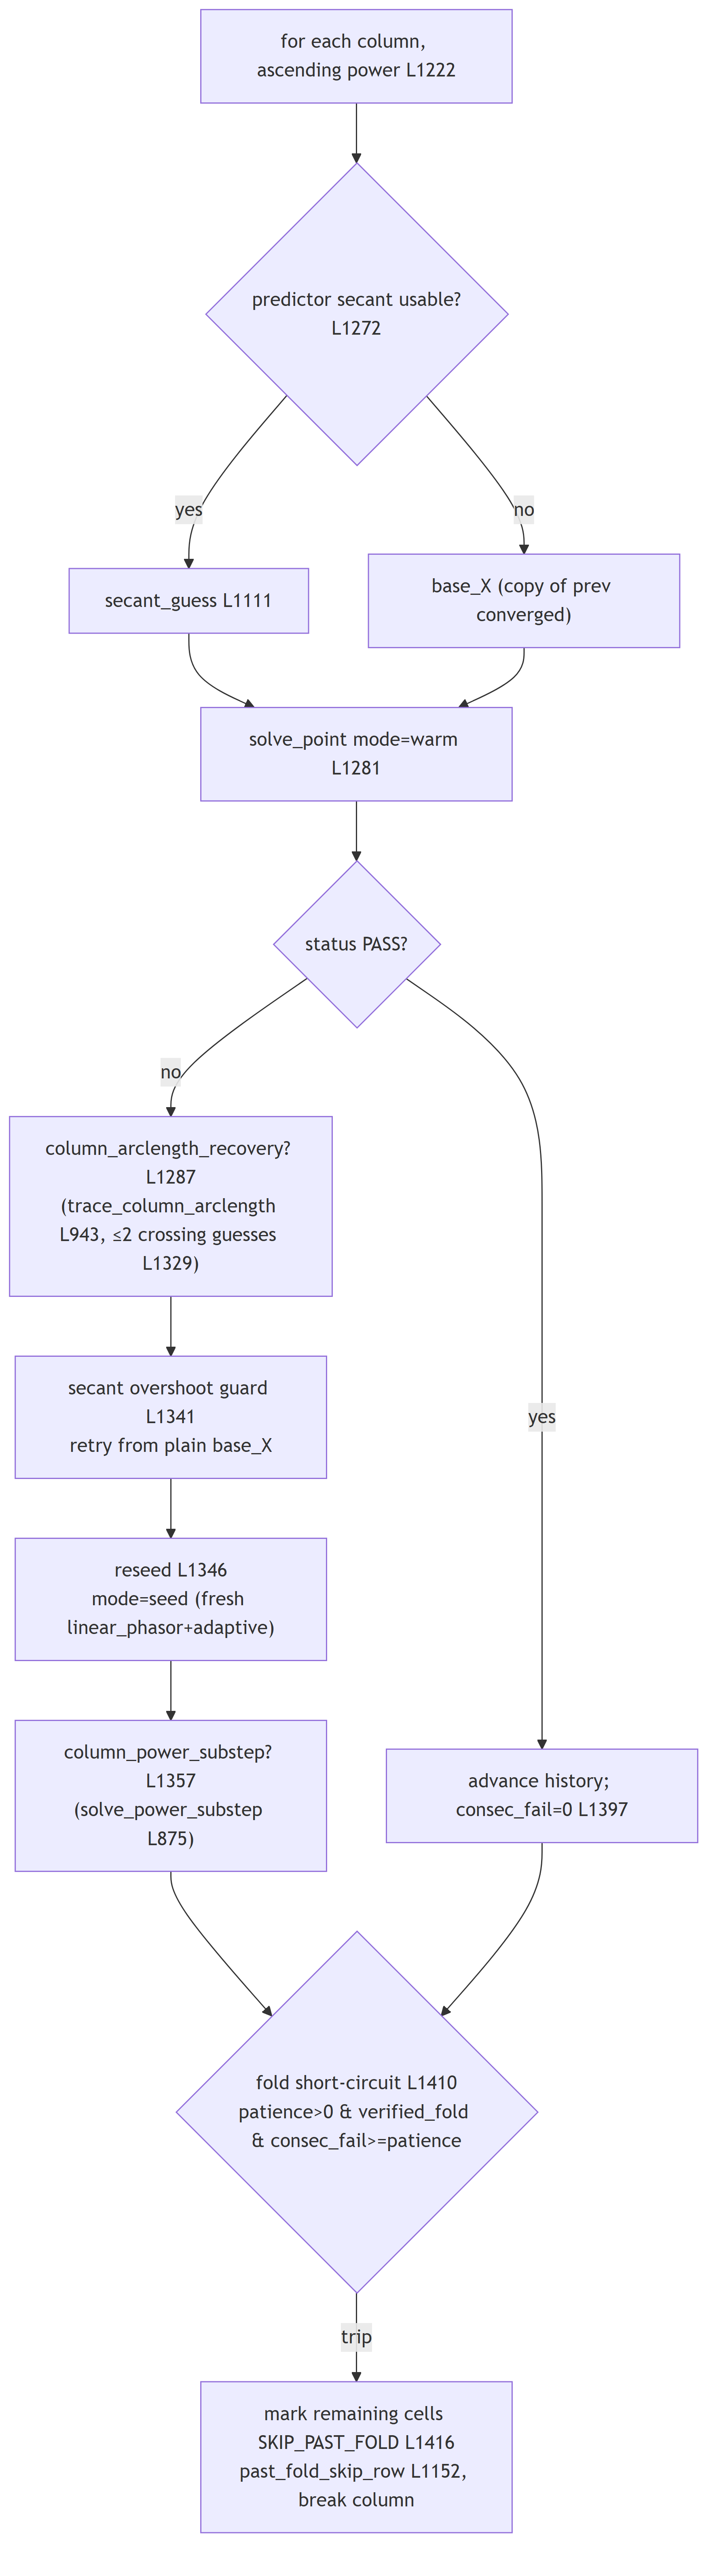
\includegraphics[width=1\linewidth,height=\textheight,keepaspectratio]{diagrams_png/diag_006.png}

\begin{itemize}
\tightlist
\item
  \texttt{-\/-inproc-fail-fast} (L1197/1263): skip reseed/substep
  recovery, keep warm-starting from the last \textbf{converged}
  neighbour (\texttt{base\_X\ =\ last\_good\_X}). One stalled solve per
  over-fold cell instead of the full recovery chain.
\item
  \texttt{-\/-initial-pump-dir} / \texttt{-\/-initial-pump-power-dbm}
  (L1217--1260): seed each column's first cell from a saved verified
  pump solution (single frequency column only, else \texttt{ValueError}
  L1218).
\end{itemize}

\subsubsection{\texorpdfstring{Power substep
(\texttt{-\/-column-power-substep})}{Power substep (-\/-column-power-substep)}}\label{power-substep---column-power-substep}

\texttt{solve\_power\_substep} (L875): adaptive natural-parameter
continuation \textbf{along the map power axis} from the last converged
state to the failed target current. Step in dBm (geometric in current
\texttt{I·10\^{}(dB/20)}), init
\texttt{-\/-column-power-substep-init-db} (0.1), grow ×1.5 / halve on
fail. If step must drop below \texttt{-\/-column-power-substep-min-db}
(0.005) → \texttt{step\_floor} terminal reason → returns \texttt{None},
sets \texttt{verified\_fold=True} and records
\texttt{pump\_power\_substep\_stall\_dbm} (L1379--1383). Bounded by
\texttt{-\/-column-power-substep-deadline-s} (120 s). A recovered
\texttt{X} re-runs \texttt{solve\_point} (L1374) so gain + files come
from the normal path.

\subsubsection{\texorpdfstring{Column arclength recovery
(\texttt{-\/-column-arclength-recovery})}{Column arclength recovery (-\/-column-arclength-recovery)}}\label{column-arclength-recovery---column-arclength-recovery}

\texttt{trace\_column\_arclength} (L943) →
\texttt{trace\_arclength\_from\_two\_points} (\texttt{solver.py} L1022):
traces one scaled pseudo-arclength branch from the last two converged
states, interpolates target-current crossings, uses up to 2 as Newton
recovery guesses. \texttt{-\/-column-arclength-ds} (0.02),
\texttt{-\/-column-arclength-max-steps} (80),
\texttt{-\/-column-arclength-deadline-s} (180). Fresh on every failing
cell (no per-column lock). A detected \texttt{fold\_lambdas} sets
\texttt{verified\_fold}.

\subsection{6.3 Inter-cell continuation (2-D traversal
orchestrator)}\label{inter-cell-continuation-2-d-traversal-orchestrator}

\texttt{run\_map\_traversal} (L1717) --- one shared
\texttt{solved{[}(i,j){]}→X} store across \textbf{both} axes; forced
single-process (\texttt{main} L2761 sets
\texttt{-\/-frequency-chunk-size\ 0}).

\begin{itemize}
\tightlist
\item
  \texttt{-\/-traversal} (\texttt{\_traversal\_order} L1439):
  \texttt{column} (col-major), \texttt{backbone} (lowest-power freq row
  first, then columns upward; \texttt{-\/-backbone-direction}
  ltr/rtl/center\_out/two\_ended L1451), \texttt{nearest} (col-major but
  recovery uses nearest solved), \texttt{serpentine} (alternating power
  direction/column), \texttt{floodfill} (Prim cheapest-neighbour from
  central low-power seed L1488).
\item
  \texttt{-\/-predictor} (\texttt{\_build\_candidates} L1525,
  \texttt{\_select\_guess} L1563): \texttt{copy},
  \texttt{power\_secant}, \texttt{freq\_secant}, \texttt{corner},
  \texttt{plane}, \texttt{portfolio} (residual-ranked via
  \texttt{predictors.rank\_candidates} L149 using
  \texttt{engine.residual\_norm} L593). \texttt{-\/-portfolio-policy}
  best\textbar ranked (ranked retries candidates in order L1753).
\item
  \texttt{-\/-recovery} (\texttt{\_recover} L1595): \texttt{none},
  \texttt{reseed} (fresh linear\_phasor+adaptive), \texttt{alt\_parent}
  (retry from power/freq/diagonal parents), \texttt{bridge}
  (\texttt{solve\_bridge} L813, physical-parameter continuation),
  \texttt{ladder} (residual-rank parents then bridge).
\item
  \texttt{-\/-fold-policy} (\texttt{\_recover} L1644): \texttt{patience}
  (count every fail), \texttt{cross\_axis}, \texttt{bridge\_gate},
  \texttt{combined} (ladder of extra rescues before counting),
  \texttt{arclength} (round the fold with \texttt{solve\_arclength}
  L1661).
\end{itemize}

\texttt{solve\_bridge} (L813) modes: \texttt{diagonal},
\texttt{freq\_first}, \texttt{power\_first}, \texttt{adaptive} (halving
step on fail, L838); \texttt{-\/-bridge-steps} (4),
\texttt{-\/-bridge-mode} (adaptive).

\begin{center}\rule{0.5\linewidth}{0.5pt}\end{center}

\section{7. Newton--Krylov iteration}\label{newtonkrylov-iteration}

One corrector call = \texttt{HarmonicNewtonKrylovSolver.solve\_one}
(\texttt{solver.py} L131--451).

\textbf{One Newton iteration.} Each iteration linearizes the residual
and solves for the update \(\Delta X\), then damps it with a
backtracking line search:

\[
J(X^{(i)})\,\Delta X = -R(X^{(i)}),
\qquad
X^{(i+1)} = X^{(i)} + \alpha\,\Delta X,\quad \alpha = 2^{-j},
\]

with \(J=\partial R/\partial X\) applied \textbf{matrix-free} (the JVP
of §4.2 --- no assembled Jacobian). The linear system is solved by
right-preconditioned GMRES,

\[
J\,M^{-1} y = -R,\qquad \Delta X = M^{-1} y ,
\]

so an approximate or stale preconditioner \(M\) (§8) only changes the
Krylov iteration count, never the converged root. Convergence is the
coefficient-relative residual
\(\lVert R\rVert_{\mathrm{coeff}} < \mathtt{newton\_tol}\) (default
\(10^{-9}\)); the line search accepts \(\alpha\) only if
\(\lVert R\rVert\) strictly decreases, and a stall detector fails the
cell if the reduction ratio stays above \(0.8\) for \(4\) consecutive
steps.

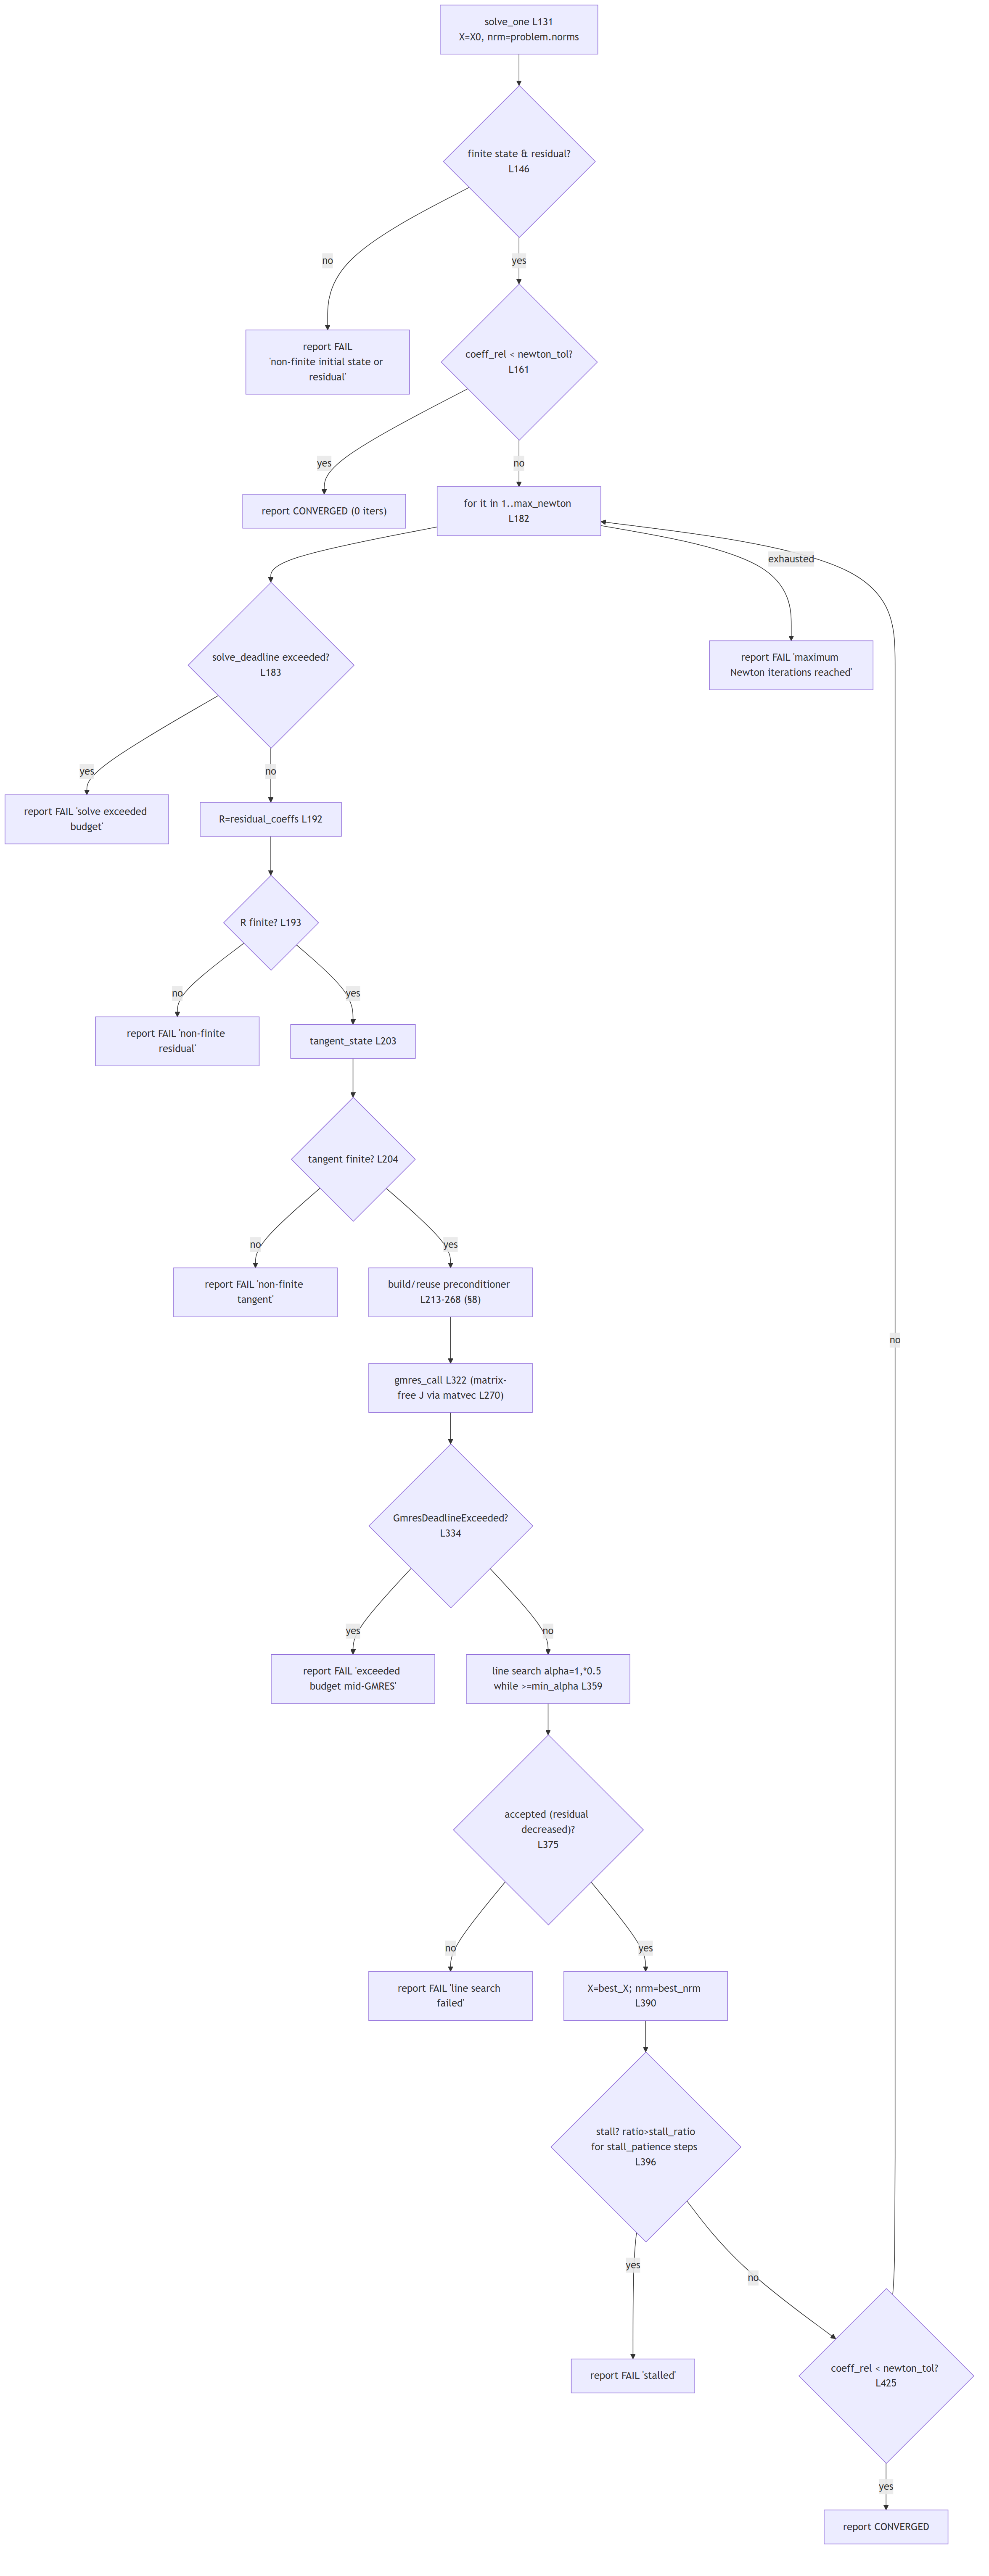
\includegraphics[width=1\linewidth,height=\textheight,keepaspectratio]{diagrams_png/diag_007.png}

\textbf{Stopping conditions and their exact origins:}

{\def\LTcaptype{none} % do not increment counter
\begin{longtable}[]{@{}
  >{\raggedright\arraybackslash}p{(\linewidth - 4\tabcolsep) * \real{0.3333}}
  >{\raggedright\arraybackslash}p{(\linewidth - 4\tabcolsep) * \real{0.3333}}
  >{\raggedright\arraybackslash}p{(\linewidth - 4\tabcolsep) * \real{0.3333}}@{}}
\toprule\noalign{}
\begin{minipage}[b]{\linewidth}\raggedright
Condition
\end{minipage} & \begin{minipage}[b]{\linewidth}\raggedright
Where
\end{minipage} & \begin{minipage}[b]{\linewidth}\raggedright
\texttt{failure\_reason} string
\end{minipage} \\
\midrule\noalign{}
\endhead
\bottomrule\noalign{}
\endlastfoot
Absolute/relative residual tol & L161, L425
(\texttt{coeff\_rel\ \textless{}\ newton\_tol}) & \texttt{""}
(converged) \\
Coefficient-relative tol & same --- \texttt{norms(){[}"coeff\_rel"{]}}
(\texttt{problem.py} L293) & --- \\
Max Newton iterations & L182 loop bound, L439 &
\texttt{maximum\ Newton\ iterations\ reached} \\
Max GMRES iterations & passed to \texttt{gmres\_call}
(\texttt{gmres\_restart=60}×\texttt{gmres\_maxiter}); \texttt{info!=0}
recorded but does \textbf{not} abort Newton (L349) &
\texttt{GMRES\ did\ not\ fully\ converge,\ info=…} \\
GMRES deadline & \texttt{gmres\_call} per-iteration callback L1194
raises \texttt{GmresDeadlineExceeded} &
\texttt{solve\ exceeded\ …s\ budget\ mid-GMRES\ at\ Newton\ \{it\}} \\
Non-finite residual (initial / mid) & L146, L193 &
\texttt{non-finite\ initial\ state\ or\ residual} /
\texttt{…residual\ before\ linear\ solve} \\
Non-finite tangent & L204 &
\texttt{non-finite\ tangent\ before\ linear\ solve} \\
Line-search exhaustion & L375
(\texttt{alpha\ \textless{}\ min\_alpha=1/1024}) &
\texttt{line\ search\ failed\ at\ Newton\ \{it\}} \\
Residual increase & handled inside line search (only accept a decrease,
L367) & --- \\
Step-size underflow & \texttt{min\_alpha} bound L359 & (→ line-search
failure) \\
Stall detector & L396--410 (\texttt{stall\_ratio=0.8},
\texttt{stall\_patience=4}) &
\texttt{stalled\ at\ Newton\ \{it\}\ (reduction\ ratio\ …)} \\
Solve deadline (per Newton) & L183 &
\texttt{solve\ exceeded\ \{…\}s\ budget\ at\ Newton\ \{it\}} \\
Backend exception (PARDISO strict) & propagates from
\texttt{\_factor}/\texttt{solve} (\texttt{fast\_coupled.py} L346/L378) &
RuntimeError (not a StepReport) \\
\end{longtable}
}

There is \textbf{no external cancellation token}; the only timeout
mechanism is \texttt{solve\_deadline\_s} (per solve) + the continuation
\texttt{max\_wall\_s}.

\begin{center}\rule{0.5\linewidth}{0.5pt}\end{center}

\section{8. Preconditioners and sparse
solvers}\label{preconditioners-and-sparse-solvers}

\texttt{-\/-inproc-preconditioner} (5 values, L2218) selects the
preconditioner built each Newton step in \texttt{solve\_one} L233--257.
All are GMRES accelerators only --- the Newton update is always against
the true matrix-free Jacobian (\texttt{matvec} L270), so a stale/approx
preconditioner never changes the converged root.

\textbf{What each preconditioner factorizes.} They differ in how much of
the mode coupling they keep. The cheap \texttt{mean\_tangent} block is
diagonal in harmonic index, using only the time-average
\(\bar\gamma=\langle\gamma(t)\rangle_t\):

\[
M_k = D_k + B_\phi\,\mathrm{diag}(\bar\gamma)\,B_\phi^{\top}.
\]

The \texttt{real\_coupled} / \texttt{real\_coupled\_fast} variants
assemble the exact mode-coupled Jacobian, where mode \(k\) couples to
mode \(q\) through the convolution harmonic \(\hat\gamma_{k-q}\)
\textbf{and} its conjugate partner \(\hat\gamma_{k+q}\) (the term
\texttt{spectral\_coupled} drops for speed):

\[
J_{k,q} = D_k\,\delta_{k,q}
        + B_\phi\,\mathrm{diag}(\hat\gamma_{k-q})\,B_\phi^{\top}
        + B_\phi\,\mathrm{diag}(\hat\gamma_{k+q})\,B_\phi^{\top}\ (\text{conjugate}) .
\]

This is real-packed as \([\mathrm{Re};\mathrm{Im}]\) and LU-factored
(PARDISO). Because it is the exact reduced Jacobian, GMRES then needs
\(\sim\!1\) iteration; \texttt{real\_coupled\_fast} additionally reuses
the symbolic factorization (fixed sparsity) so only the numeric phase
repeats.

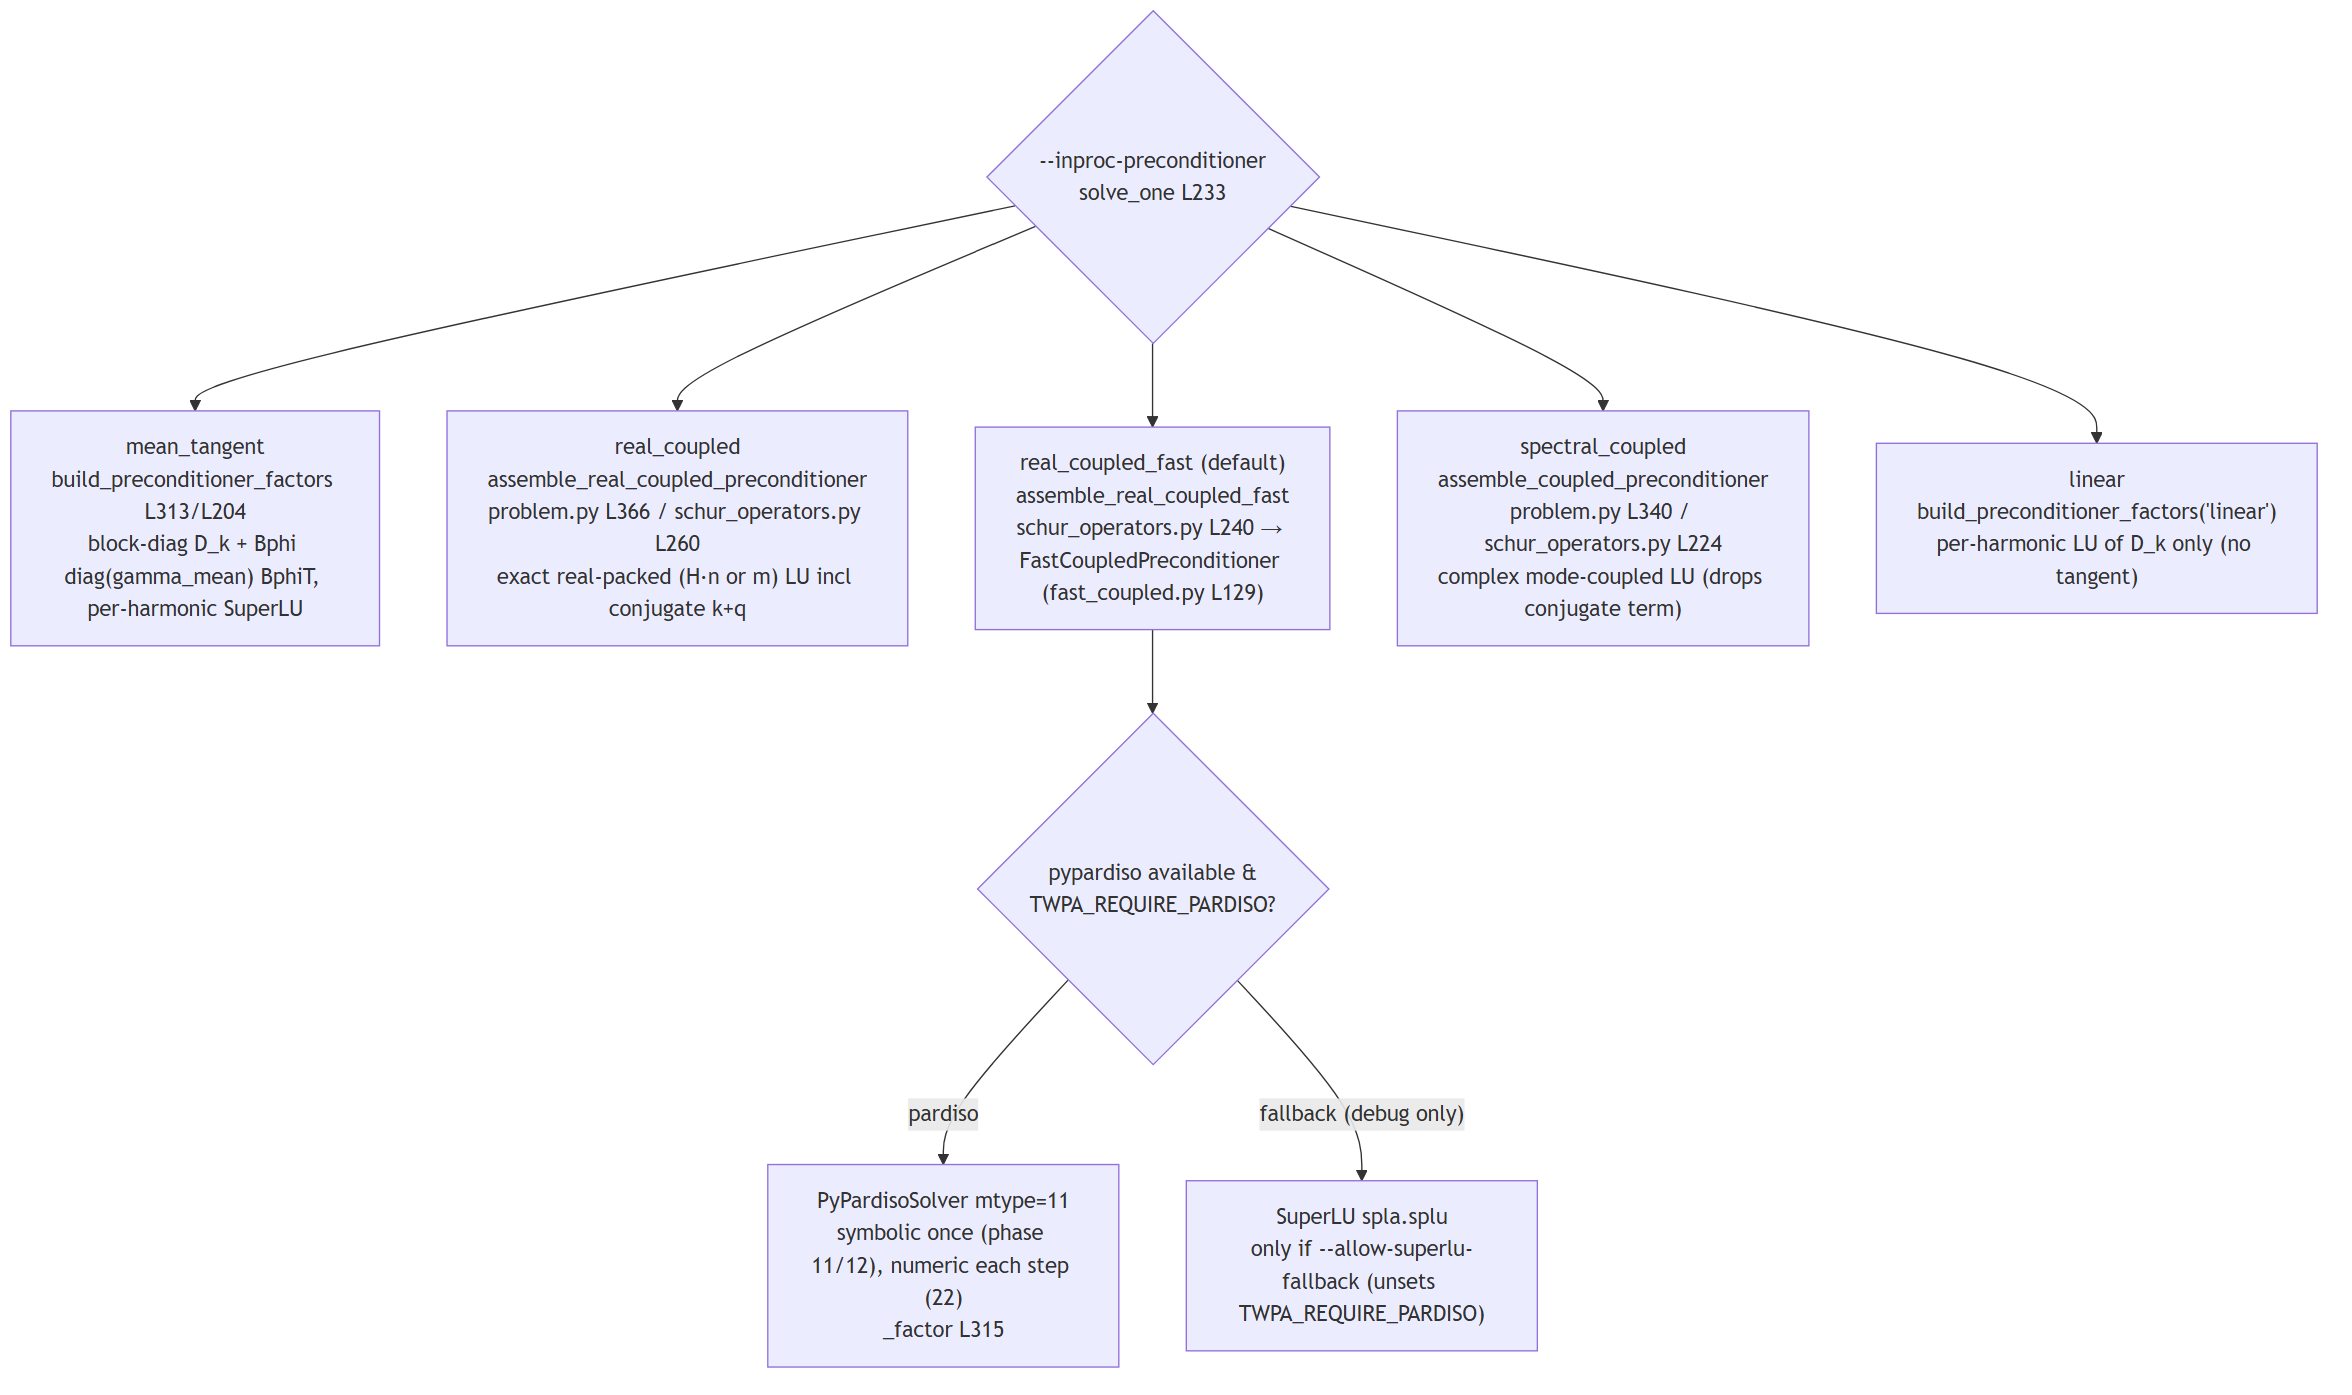
\includegraphics[width=1\linewidth,height=\textheight,keepaspectratio]{diagrams_png/diag_008.png}

{\def\LTcaptype{none} % do not increment counter
\begin{longtable}[]{@{}
  >{\raggedright\arraybackslash}p{(\linewidth - 10\tabcolsep) * \real{0.1667}}
  >{\raggedright\arraybackslash}p{(\linewidth - 10\tabcolsep) * \real{0.1667}}
  >{\raggedright\arraybackslash}p{(\linewidth - 10\tabcolsep) * \real{0.1667}}
  >{\raggedright\arraybackslash}p{(\linewidth - 10\tabcolsep) * \real{0.1667}}
  >{\raggedright\arraybackslash}p{(\linewidth - 10\tabcolsep) * \real{0.1667}}
  >{\raggedright\arraybackslash}p{(\linewidth - 10\tabcolsep) * \real{0.1667}}@{}}
\toprule\noalign{}
\begin{minipage}[b]{\linewidth}\raggedright
CLI value
\end{minipage} & \begin{minipage}[b]{\linewidth}\raggedright
Matrix factorized
\end{minipage} & \begin{minipage}[b]{\linewidth}\raggedright
Symbolic reuse
\end{minipage} & \begin{minipage}[b]{\linewidth}\raggedright
Numeric refactor
\end{minipage} & \begin{minipage}[b]{\linewidth}\raggedright
GMRES convergence
\end{minipage} & \begin{minipage}[b]{\linewidth}\raggedright
Notes / restrictions
\end{minipage} \\
\midrule\noalign{}
\endhead
\bottomrule\noalign{}
\endlastfoot
\texttt{mean\_tangent} & \texttt{D\_k\ +\ Bphiᵀ·diag(γ\_mean)·Bphi} per
harmonic (block-diag) & none (fresh \texttt{splu} each step) & every
step & several iters & cheapest for tiny warm-start steps \\
\texttt{real\_coupled} & exact real-packed \texttt{(2·H·n)} Jacobian
incl.~conjugate \texttt{K\_\{k+q\}}
(\texttt{\_build\_real\_coupled\_matrix} L372) & none & every step &
\textasciitilde1 iter & full backend only; costly LU \\
\texttt{real\_coupled\_fast} (default) & same exact matrix, but assembly
via precomputed scatter map + \textbf{symbolic-factorization reuse}
(\texttt{FastCoupledPreconditioner}) & \textbf{yes} (PARDISO phase 11
once/partition; scatter map cached on partition) & numeric phase 22 each
step & \textasciitilde1 iter & \textbf{Schur backend only} --- raises
\texttt{NotImplementedError} on \texttt{full} (\texttt{solve\_one}
L242) \\
\texttt{spectral\_coupled} & complex mode-coupled \texttt{(H·n)} LU,
drops conjugate \texttt{k+q} term
(\texttt{assemble\_coupled\_preconditioner} L340) & none & every step &
few iters & near-exact for weak conjugate coupling \\
\texttt{linear} & \texttt{D\_k} only, per harmonic & none & once
(X-independent) but rebuilt per step in loop & many iters & ignores
nonlinearity \\
\end{longtable}
}

\textbf{Reuse policy (\texttt{-\/-inproc-precond-reuse},
\texttt{-\/-inproc-precond-refresh-gmres}).} \texttt{solve\_one}
L217--223 decides \texttt{refresh}: rebuild if no cache,
\texttt{precond\_reuse\ ≤\ 1},
\texttt{steps\_since\_factor\ ≥\ precond\_reuse}, or previous GMRES
iters \texttt{≥\ refresh\_gmres}. Reuse trades extra GMRES iters for
skipping the LU rebuild (modified-Newton). Default
\texttt{precond\_reuse=1} refactors every step.

\textbf{Sparse factorization libraries:}

\begin{itemize}
\tightlist
\item
  \textbf{SuperLU} (\texttt{scipy.sparse.linalg.splu}): mean\_tangent /
  spectral\_coupled / real\_coupled / linear factor with SuperLU; the
  Schur \texttt{D\_ee} blocks (\texttt{schur\_partition.py} L128) and
  signal \texttt{superlu} path (\texttt{floquet.py} L200).
\item
  \textbf{MKL PARDISO} (\texttt{pypardiso}):
  \texttt{real\_coupled\_fast} (\texttt{fast\_coupled.py}
  \texttt{\_factor} L315) and the signal \texttt{pardiso} path
  (\texttt{\_pardiso\_spsolve\_reuse} L59). Both single-thread the BLAS
  via \texttt{\_pardiso\_thread\_context} (env
  \texttt{TWPA\_PARDISO\_THREADS}, default 1) to dodge a Windows MKL
  reordering failure (error −3).
\end{itemize}

\textbf{PARDISO strictness / telemetry.} \texttt{main} L2749--2755 sets
\texttt{TWPA\_REQUIRE\_PARDISO=1} unless
\texttt{-\/-allow-superlu-fallback}, and \texttt{TWPA\_PARDISO\_LOG=1}
if \texttt{-\/-log-factor-backend}. Under strict mode a PARDISO failure
\textbf{raises} (\texttt{fast\_coupled.py} L346/L378) rather than
silently downgrading. Telemetry: \texttt{last\_assembly\_runtime\_s},
\texttt{last\_factor\_runtime\_s}, \texttt{last\_factor\_backend} on the
preconditioner, surfaced into the row as
\texttt{pump\_preconditioner\_assembly\_runtime\_s} /
\texttt{…\_numeric\_factor\_runtime\_s} (solve\_point L756--757, sourced
solver.py L266--268).

\textbf{Matrix-free advanced-continuation path.}
\texttt{\_linear\_solver} (\texttt{solver.py} L736) always uses the
exact real-coupled factor (\texttt{assemble\_real\_coupled\_fast} if
Schur, else \texttt{assemble\_real\_coupled\_preconditioner}) regardless
of \texttt{-\/-inproc-preconditioner} --- the tangent/PTC/arclength
solves are near-direct.

\begin{center}\rule{0.5\linewidth}{0.5pt}\end{center}

\section{9. Signal-side factor solve
(detailed)}\label{signal-side-factor-solve-detailed}

\textbf{The linear Floquet problem.} The converged pump fixes
\(\gamma(t)=\cos\!\big(\psi_p(t)/\phi_0\big)\,I_c/\phi_0\); its Fourier
harmonics \(\hat\gamma_\ell\) build the parametric coupling matrices

\[
\hat K_\ell = B_\phi\,\mathrm{diag}(\hat\gamma_\ell)\,B_\phi^{\top}.
\]

A small signal at \(\omega_s\) scatters into sidebands
\(m\in\{-S,\dots,S\}\) at \(\omega_s+m\omega_p\). These are coupled by
the block \textbf{conversion matrix}, giving one linear system per
signal frequency (no nonlinear iteration):

\[
A_{m,q} = \hat K_{m-q} + \delta_{m,q}\,D\!\big(\omega_s + m\omega_p\big),
\qquad
A\,\Phi = b ,
\]

where \(D(\omega)=K-\omega^2 C + i\omega G\) is the linear node
admittance and the RHS \(b\) injects a unit current at the source port
in the signal sideband \(m=0\). The output port flux gives the wave and
the scattering parameter, hence the gain in dB:

\[
v_{\mathrm{out}} = i\,\omega_s\,\phi_{\mathrm{out}},
\qquad
G_{\mathrm{dB}} = 20\,\log_{10}\big\lvert S_{\mathrm{out,src}}\big\rvert .
\]

The \texttt{schur} backend applies the same reduction as §4.3 to \(A\)
before solving; the two baseline solves (pump off, pump-diagonal) reuse
\(\hat K\) at \(\ell=0\) to normalize the gain.

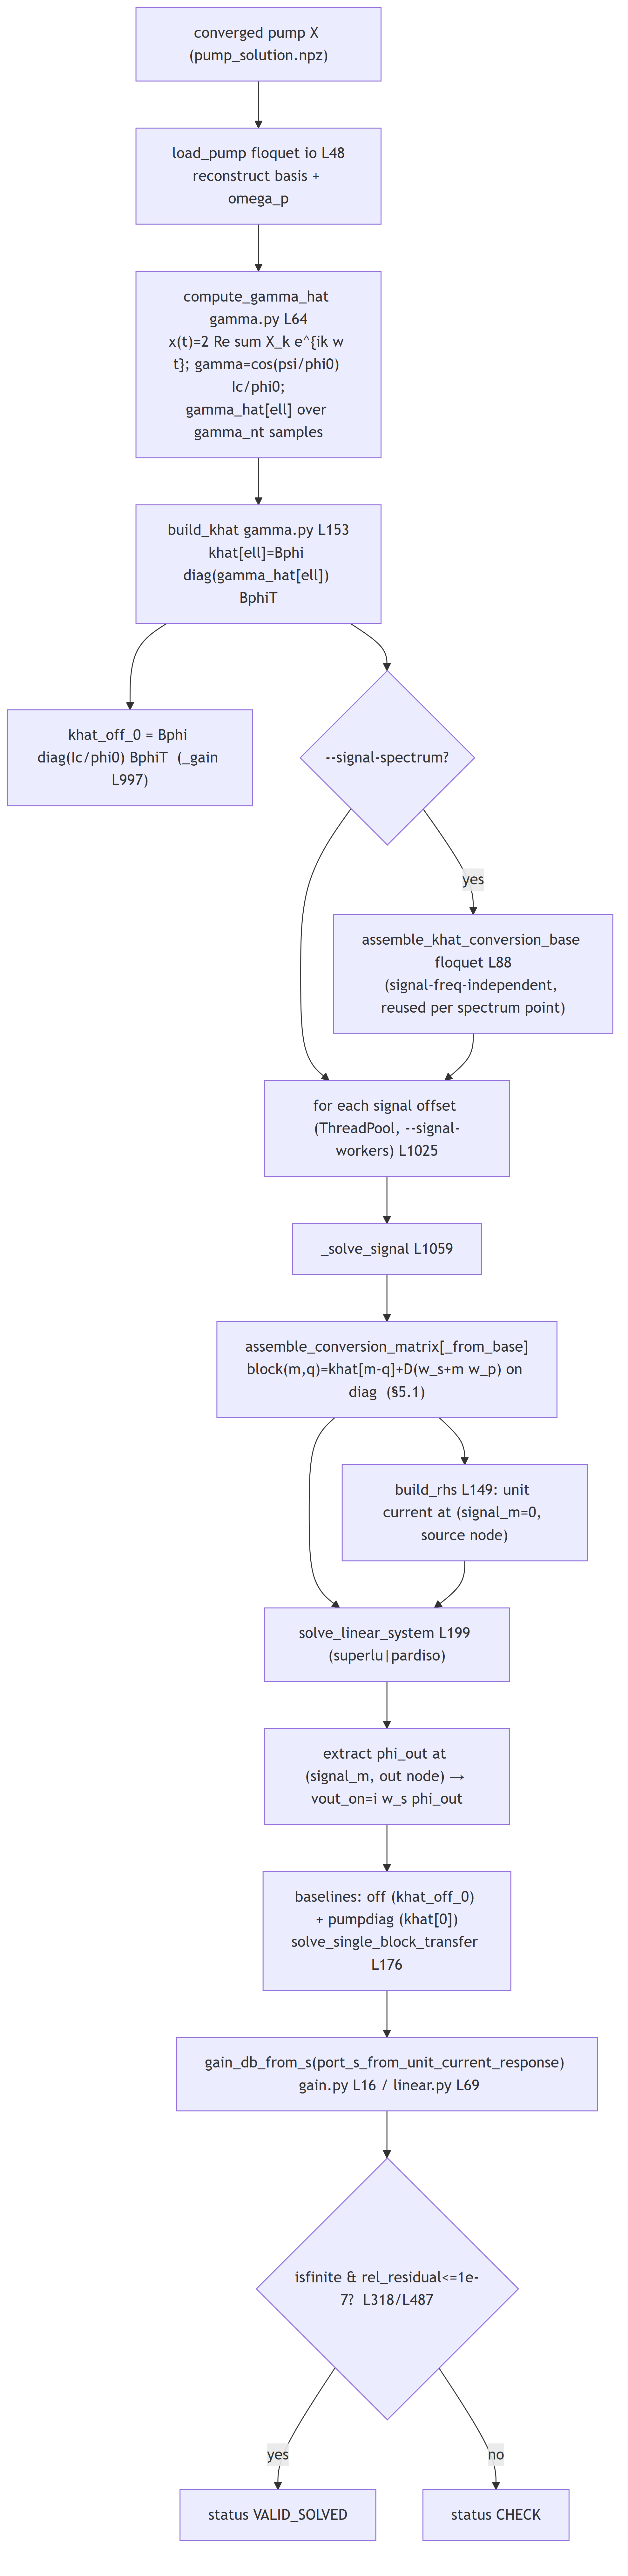
\includegraphics[width=1\linewidth,height=\textheight,keepaspectratio]{diagrams_png/diag_009.png}

\textbf{Loops involved:}

\begin{itemize}
\tightlist
\item
  \textbf{Pump map cells:} \texttt{run\_warm\_pass\_inprocess} /
  \texttt{run\_map\_traversal} iterate cells; each converged (or
  \texttt{force\_gain}) cell calls \texttt{\_gain} (solve\_point L786).
\item
  \textbf{Signal frequencies:} spectrum offsets
  \texttt{spectrum\_offsets\_mhz} (L121), looped in \texttt{\_gain}
  L1016--1039; plus one trailing target signal (L1041).
\item
  \textbf{Worker threads:}
  \texttt{ThreadPoolExecutor(-\/-signal-workers)} over offsets (L1026).
\item
  \textbf{Sidebands:} implicit in the \texttt{(2S+1)} block assembly
  (\texttt{sideband\_list}, L84).
\item
  \textbf{Ports:} fixed \texttt{source\_port}/\texttt{out\_port}; RHS
  built at the source, output read at the out node (\texttt{build\_rhs}
  L149, \texttt{extract\_sideband\_node} L162).
\item
  \textbf{Shared factorization:} \texttt{khat\_big\_base} (spectrum) and
  the signal Schur \textbf{partition} cache (per (ω\_p, ω\_s, S, ports),
  L1063) amortize assembly; there is \textbf{no} shared LU across signal
  frequencies (each \texttt{A(ω\_s)} differs), unlike the pump
  \texttt{D\_ee} reuse.
\end{itemize}

\texttt{load\_pump} upcasts the float32-stored \texttt{X} back to
complex128 (\texttt{load\_pump\_basis\_from\_solution} L264) so float32
storage never leaks complex64 into scipy.

\begin{center}\rule{0.5\linewidth}{0.5pt}\end{center}

\section{10. Fold detection and fold
recovery}\label{fold-detection-and-fold-recovery}

There is \textbf{no single fold flag}; ``fold'' is inferred through
several paths and only the \texttt{arclength}/substep paths
\emph{confirm} a turning point, versus a mere numerical failure.

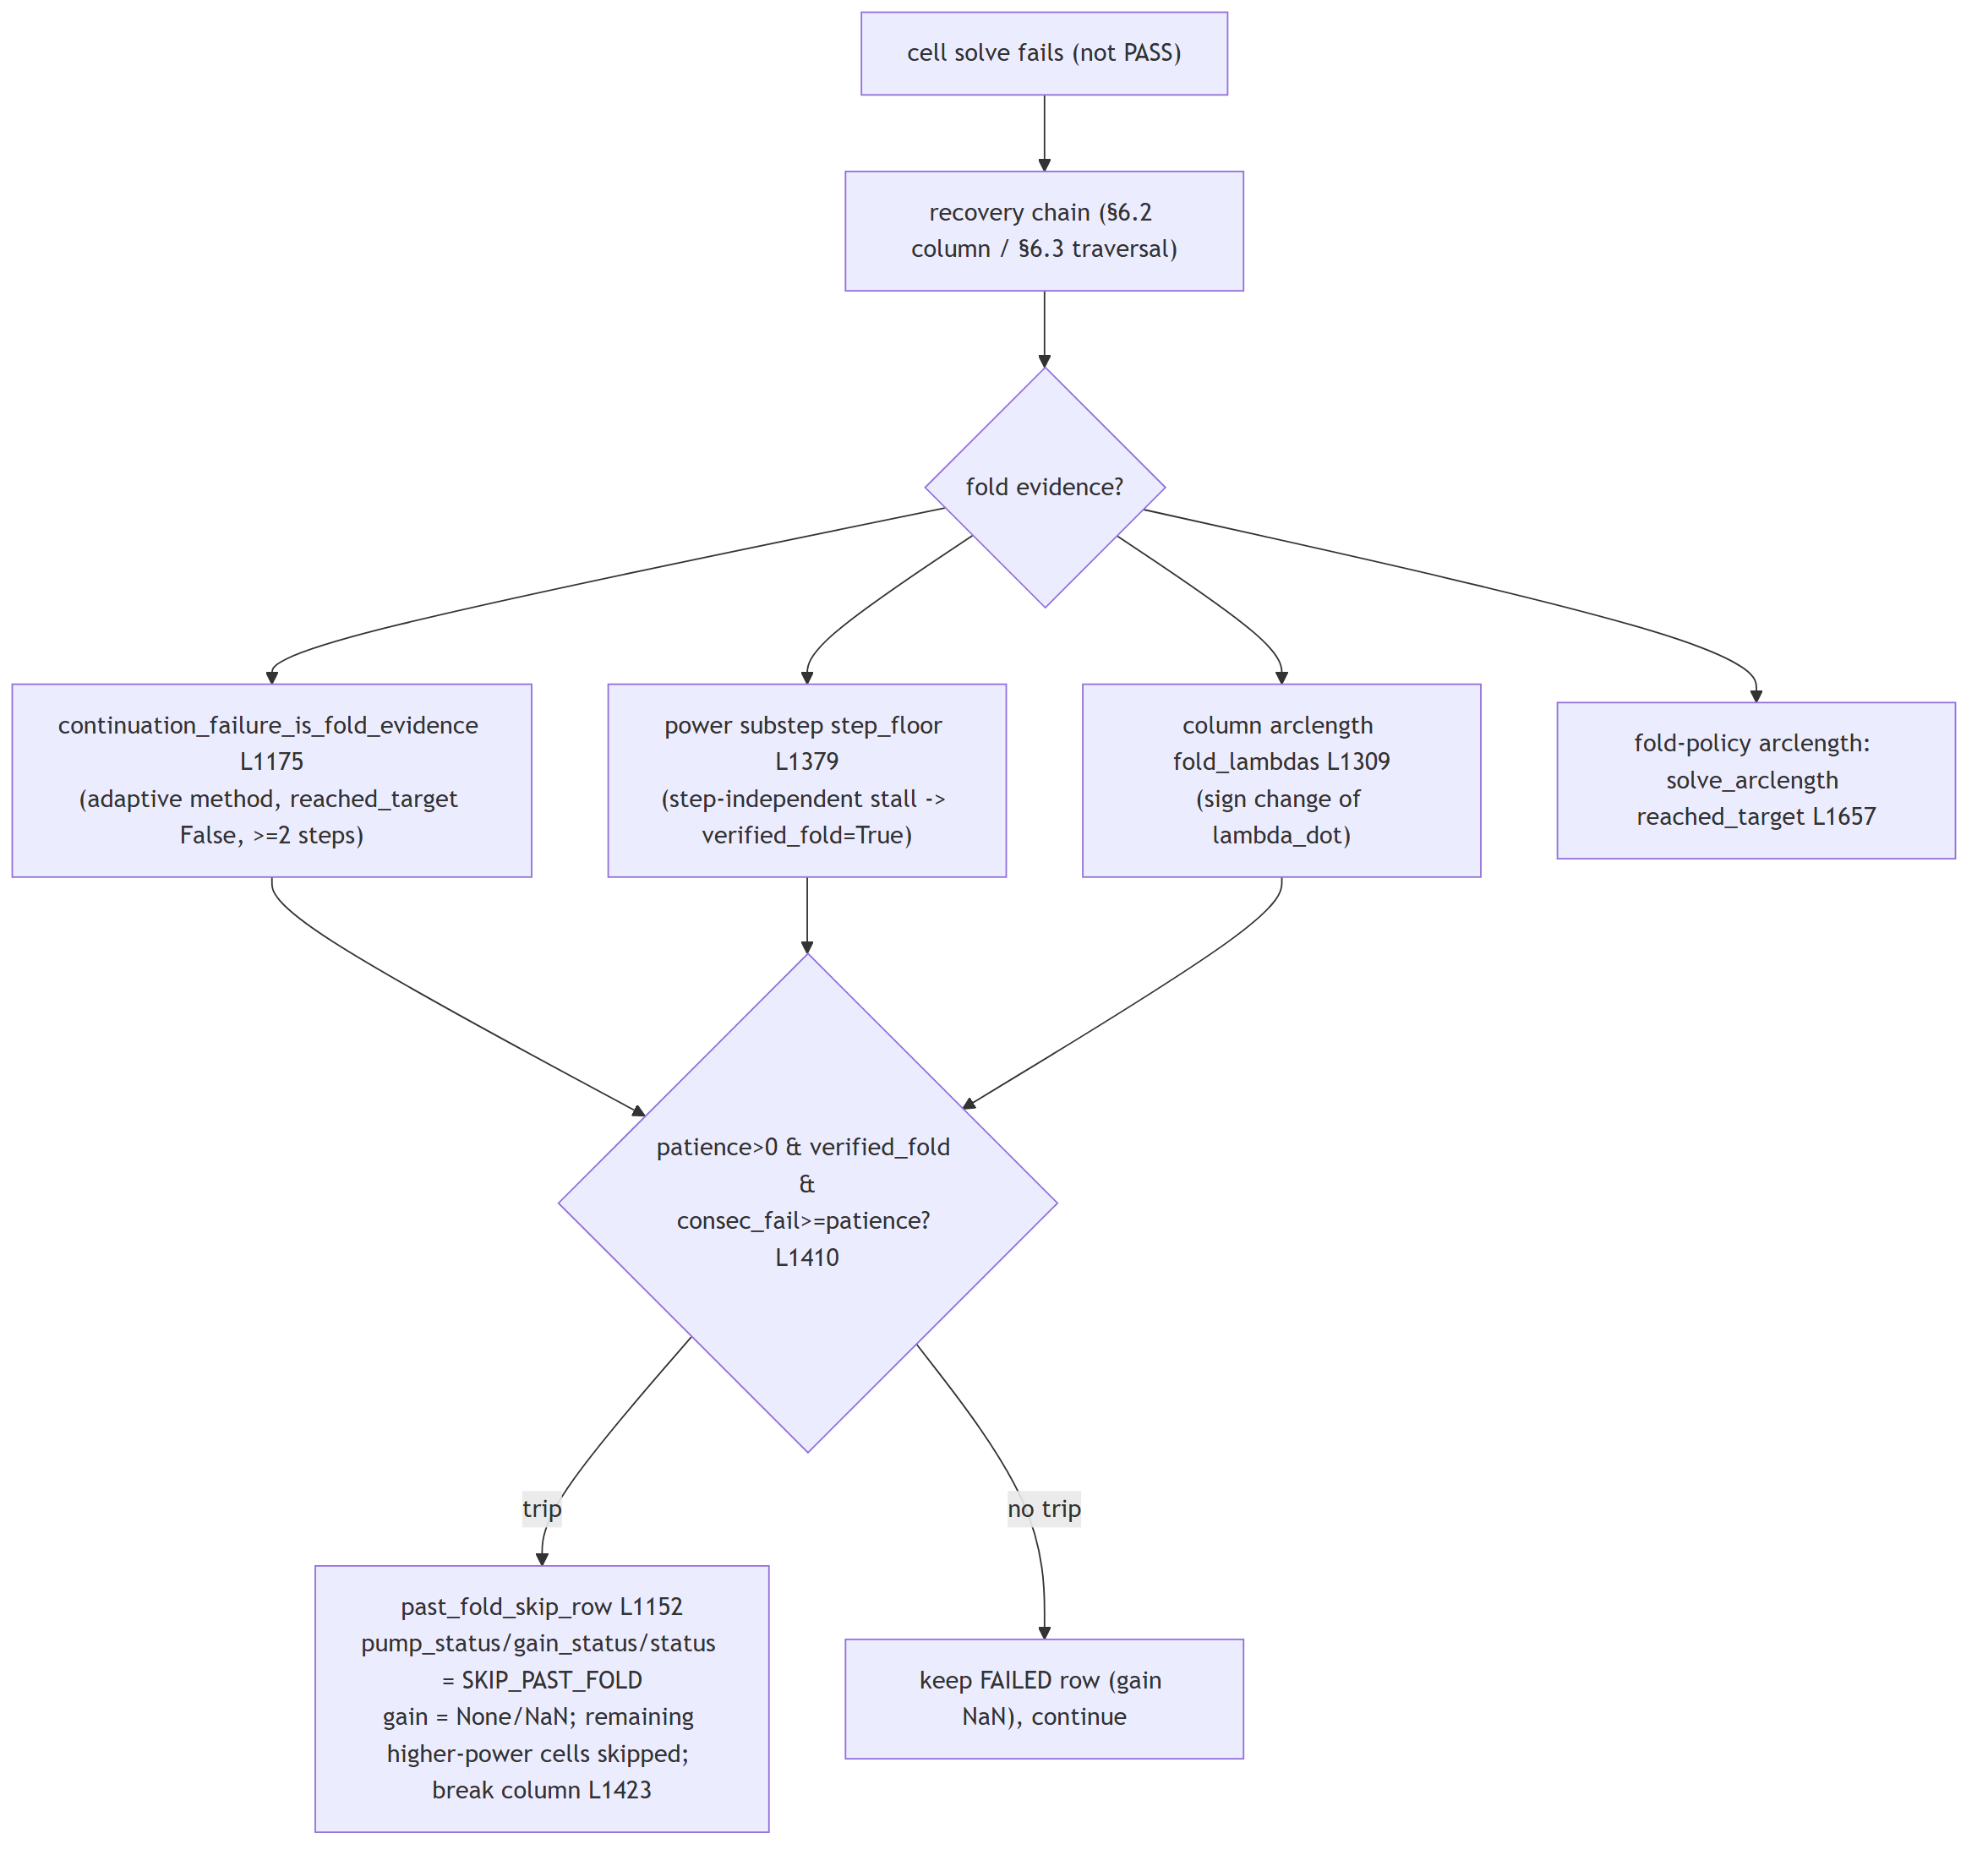
\includegraphics[width=1\linewidth,height=\textheight,keepaspectratio]{diagrams_png/diag_010.png}

\begin{itemize}
\tightlist
\item
  \textbf{Predictor failure near fold:} secant overshoot guard retries
  from the plain warm start (\texttt{run\_warm\_pass\_inprocess} L1341).
\item
  \textbf{Newton failure near fold:} stall detector / deadline in
  \texttt{solve\_one} fail the cell fast (§7), avoiding thousands of
  GMRES iters.
\item
  \textbf{Retry from plain warm start / reseed:} L1342 / L1346.
\item
  \textbf{Tangent/mean-tangent recovery:} via
  \texttt{-\/-inproc-continuation\ adaptive\_tangent}
  (tangent\_predictor) or the mean\_tangent preconditioner; no dedicated
  ``tangent recovery'' path beyond these.
\item
  \textbf{Pseudo-arclength path:} \texttt{-\/-column-arclength-recovery}
  (column) and \texttt{-\/-fold-policy\ arclength} (traversal).
\item
  \textbf{Fixed continuation fallback:} inside
  \texttt{solve\_adaptive\_continuation} when the step floor is hit
  (L682).
\item
  \textbf{Fold-skip patience counter:} \texttt{-\/-fold-skip-patience}
  (default 0 = disabled). In the legacy column pass the skip requires
  \textbf{both} \texttt{consec\_fail\ ≥\ patience} \textbf{and}
  \texttt{verified\_fold} (L1410) --- a bare failed solve is never
  treated as a fold. In \texttt{run\_map\_traversal} (L1785) the
  traversal short-circuit uses \texttt{col\_fail{[}j{]}\ ≥\ patience}
  \textbf{without} the \texttt{verified\_fold} gate (a documented
  asymmetry, see §14).
\item
  \textbf{\texttt{SKIP\_PAST\_FOLD}:} the string constant (L1133); rows
  via \texttt{past\_fold\_skip\_row} (L1152). Gain is \texttt{None} in
  the row → \texttt{NaN} in the grid (\texttt{gain\_grid} L1938).
\item
  \textbf{False-fold risk:} a small \texttt{-\/-inproc-max-newton} /
  short \texttt{-\/-inproc-solve-deadline-s} makes a solvable-but-stiff
  cell fail; combined with traversal patience (no
  \texttt{verified\_fold} gate) this can skip a real operating region.
  Documented in the memory \texttt{foldskip-culls-broadband-2c}.
\item
  \textbf{Numerical failure vs confirmed fold:} only
  \texttt{verified\_fold} (substep step\_floor, arclength sign change)
  marks a confirmed turning point; everything else is a numerical
  failure (\texttt{FAIL}, gain NaN, retryable).
\item
  \textbf{\texttt{-\/-fold-follow}} (\texttt{run\_fold\_follow} L1680)
  is a separate diagnostic mode: at each frequency it builds the
  max-power problem and calls \texttt{fold\_power} (\texttt{solver.py}
  L1225, pseudo-arclength from λ=0 until the first \texttt{λ\_dot} sign
  change) → \texttt{fold\_curve.csv}. No gain map is produced
  (\texttt{main} L2786--2791).
\end{itemize}

\begin{center}\rule{0.5\linewidth}{0.5pt}\end{center}

\section{11. Status propagation (state
machine)}\label{status-propagation-state-machine}

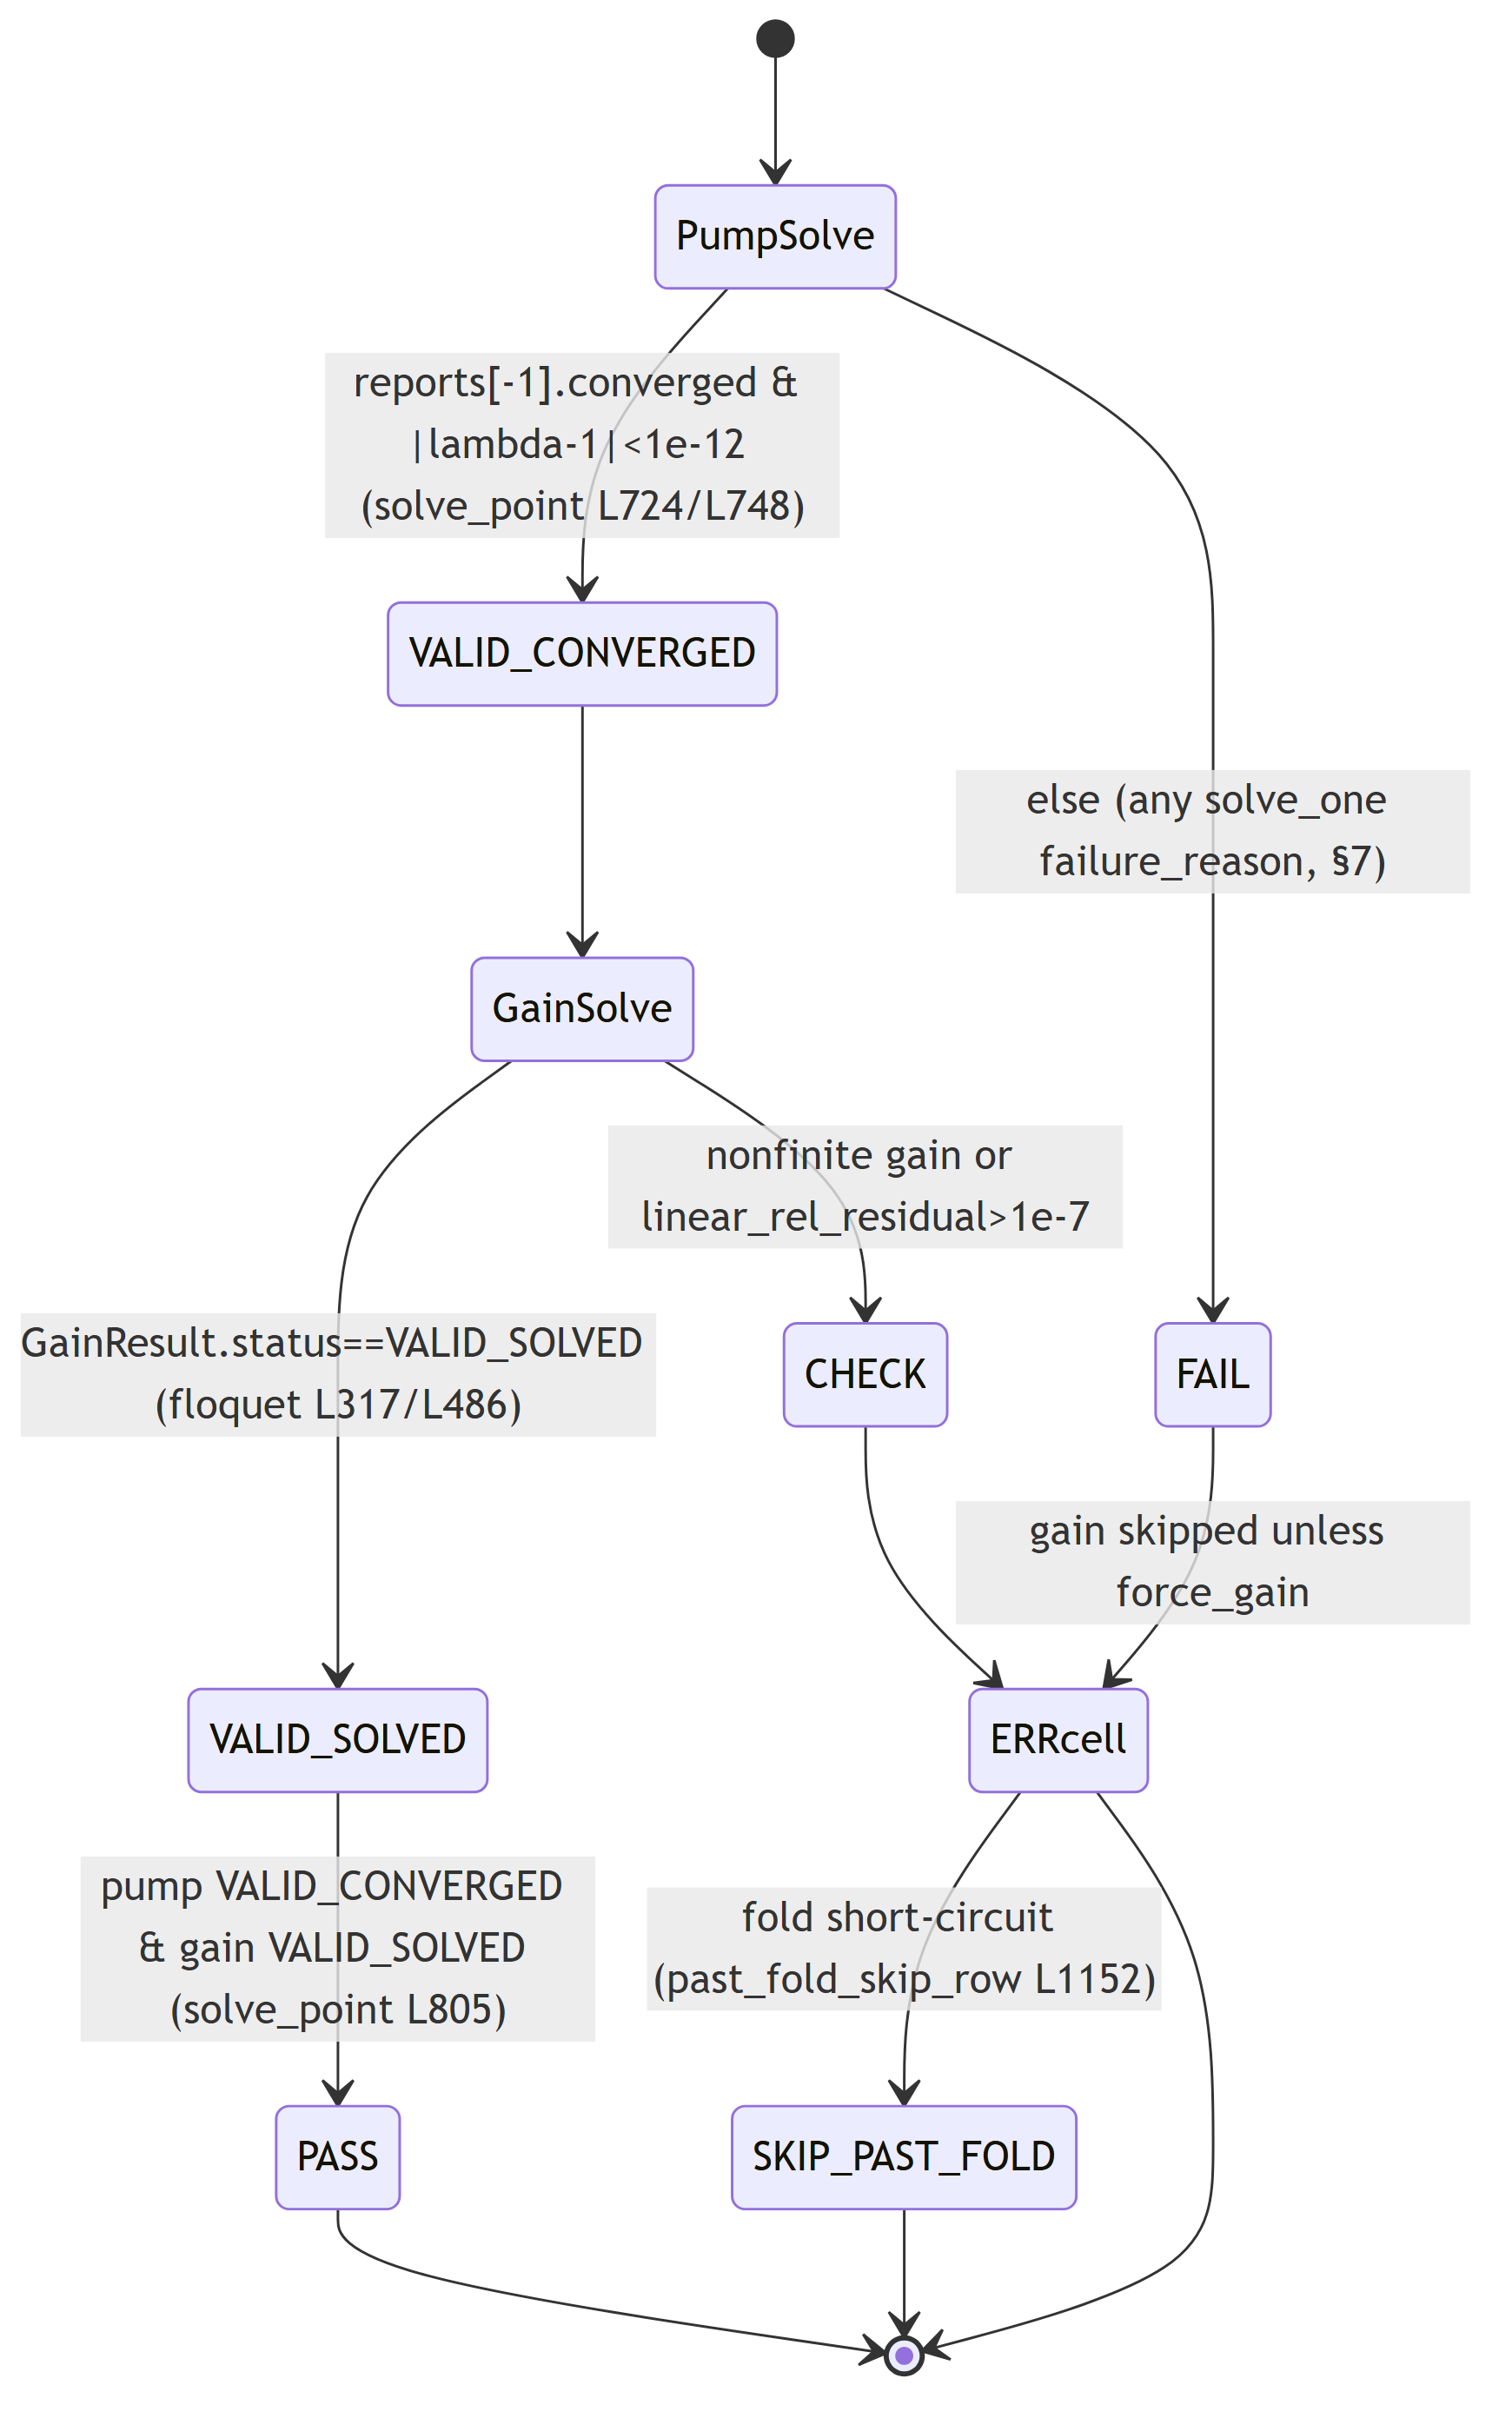
\includegraphics[width=1\linewidth,height=\textheight,keepaspectratio]{diagrams_png/diag_011.png}

Exact status strings found in the implementation and their handling:

{\def\LTcaptype{none} % do not increment counter
\begin{longtable}[]{@{}
  >{\raggedright\arraybackslash}p{(\linewidth - 16\tabcolsep) * \real{0.1111}}
  >{\raggedright\arraybackslash}p{(\linewidth - 16\tabcolsep) * \real{0.1111}}
  >{\raggedright\arraybackslash}p{(\linewidth - 16\tabcolsep) * \real{0.1111}}
  >{\raggedright\arraybackslash}p{(\linewidth - 16\tabcolsep) * \real{0.1111}}
  >{\raggedright\arraybackslash}p{(\linewidth - 16\tabcolsep) * \real{0.1111}}
  >{\raggedright\arraybackslash}p{(\linewidth - 16\tabcolsep) * \real{0.1111}}
  >{\raggedright\arraybackslash}p{(\linewidth - 16\tabcolsep) * \real{0.1111}}
  >{\raggedright\arraybackslash}p{(\linewidth - 16\tabcolsep) * \real{0.1111}}
  >{\raggedright\arraybackslash}p{(\linewidth - 16\tabcolsep) * \real{0.1111}}@{}}
\toprule\noalign{}
\begin{minipage}[b]{\linewidth}\raggedright
Status
\end{minipage} & \begin{minipage}[b]{\linewidth}\raggedright
Created at
\end{minipage} & \begin{minipage}[b]{\linewidth}\raggedright
Condition
\end{minipage} & \begin{minipage}[b]{\linewidth}\raggedright
Retryable?
\end{minipage} & \begin{minipage}[b]{\linewidth}\raggedright
Triggers fallback?
\end{minipage} & \begin{minipage}[b]{\linewidth}\raggedright
Terminates
\end{minipage} & \begin{minipage}[b]{\linewidth}\raggedright
Gain computed?
\end{minipage} & \begin{minipage}[b]{\linewidth}\raggedright
Written
\end{minipage} & \begin{minipage}[b]{\linewidth}\raggedright
Exit code
\end{minipage} \\
\midrule\noalign{}
\endhead
\bottomrule\noalign{}
\endlastfoot
\texttt{VALID\_CONVERGED} (pump) & solve\_point L748; write\_results L62
& converged at λ=1 & --- & --- & --- & yes & \texttt{pump\_status} col,
\texttt{pump\_report.json\ final\_status} & --- \\
\texttt{FAIL} (pump) & solve\_point L748; write\_results L64 & any
\texttt{solve\_one} non-converge & yes (recovery chain) & yes & cell &
no (unless \texttt{force\_gain}) & \texttt{pump\_status},
\texttt{pump\_failure\_reason} & --- \\
\texttt{VALID\_SOLVED} (gain) & \texttt{GainResult} floquet L317/L486 &
finite gain, resid≤1e-7 & --- & --- & --- & yes & \texttt{gain\_status},
\texttt{gain\_db} & --- \\
\texttt{CHECK} (gain) & floquet L318/L487 & nonfinite or
resid\textgreater1e-7 & (not retried) & no & cell →
\texttt{gain\_status=ERROR} in row unless VALID\_SOLVED & yes but
suspect & \texttt{gain\_status} (mapped to ERROR at L781/L798) & --- \\
\texttt{PASS} (cell) & solve\_point L805 & pump VALID\_CONVERGED
\textbf{and} gain VALID\_SOLVED & --- & --- & --- & yes &
\texttt{status} col & --- \\
\texttt{ERROR} (cell) & solve\_point L781/L806 & anything else &
(recovery already ran) & --- & cell & maybe & \texttt{status} col &
--- \\
\texttt{SKIP\_PAST\_FOLD} & L1133 / \texttt{past\_fold\_skip\_row} L1152
& patience trip past a verified fold & no (intentional) & no & remaining
higher-power cells in column & no (NaN) &
\texttt{status}/\texttt{pump\_status}/\texttt{gain\_status},
\texttt{pump\_failure\_reason} & --- \\
GMRES/line-search/stall/deadline/nonfinite & \texttt{failure\_reason}
strings inside \texttt{StepReport} (§7) & see §7 table & --- & --- &
rolls up into pump \texttt{FAIL} & --- & \texttt{pump\_failure\_reason}
col + \texttt{pump\_report.json\ reports{[}{]}} & --- \\
\end{longtable}
}

\textbf{Note on naming.} The task's example enum names
(\texttt{CONVERGED}, \texttt{SOLVED}, \texttt{GMRES\_FAILED},
\texttt{LINE\_SEARCH\_FAILED}, \texttt{MAX\_NEWTON}, \texttt{DEADLINE},
\texttt{STALL}, \texttt{NONFINITE}, \texttt{UNSUPPORTED\_BACKEND},
\texttt{INVALID\_CONFIGURATION}, \texttt{MISSING\_SEED},
\texttt{PARTIAL}) are \textbf{not} literal strings in the code. The
implementation uses: pump \texttt{VALID\_CONVERGED}/\texttt{FAIL}, gain
\texttt{VALID\_SOLVED}/\texttt{CHECK}, cell
\texttt{PASS}/\texttt{ERROR}/\texttt{SKIP\_PAST\_FOLD}, plus free-text
\texttt{failure\_reason} phrases (e.g.~\texttt{stalled\ at\ Newton\ …},
\texttt{line\ search\ failed\ at\ Newton\ …},
\texttt{maximum\ Newton\ iterations\ reached},
\texttt{solve\ exceeded\ …s\ budget\ …}, \texttt{non-finite\ …},
\texttt{GMRES\ did\ not\ fully\ converge,\ info=…}). ``Unsupported
backend'' surfaces as a raised
\texttt{NotImplementedError}/\texttt{ValueError}, never a status string.

\textbf{Process exit codes} (\texttt{main} L2891--2893): \texttt{1} iff
a gate was evaluated and failed; else \texttt{0}. A chunk worker failure
raises \texttt{RuntimeError} (\texttt{run\_frequency\_chunks} L2740) →
non-zero via the unhandled exception. \texttt{-\/-fold-follow} returns
\texttt{0} (L2791). Per-cell FAIL does \textbf{not} by itself set a
non-zero exit.

\begin{center}\rule{0.5\linewidth}{0.5pt}\end{center}

\section{12. CLI option inventory}\label{cli-option-inventory}

\texttt{Scope} codes: \textbf{Pump}, \textbf{Signal}, \textbf{Cont}
(continuation), \textbf{Precond}, \textbf{Sparse}, \textbf{Trav} (map
traversal), \textbf{Par} (parallelism), \textbf{Out}, \textbf{Recov},
\textbf{Res} (resource limits), \textbf{Exec}.

All rows are from \texttt{run\_gain\_map.parse\_args} (L2111--2451)
unless noted. Full machine-readable form: \texttt{cli\_inventory.csv} /
\texttt{cli\_inventory.json}.

{\def\LTcaptype{none} % do not increment counter
\begin{longtable}[]{@{}
  >{\raggedright\arraybackslash}p{(\linewidth - 12\tabcolsep) * \real{0.1429}}
  >{\raggedright\arraybackslash}p{(\linewidth - 12\tabcolsep) * \real{0.1429}}
  >{\raggedright\arraybackslash}p{(\linewidth - 12\tabcolsep) * \real{0.1429}}
  >{\raggedright\arraybackslash}p{(\linewidth - 12\tabcolsep) * \real{0.1429}}
  >{\raggedright\arraybackslash}p{(\linewidth - 12\tabcolsep) * \real{0.1429}}
  >{\raggedright\arraybackslash}p{(\linewidth - 12\tabcolsep) * \real{0.1429}}
  >{\raggedright\arraybackslash}p{(\linewidth - 12\tabcolsep) * \real{0.1429}}@{}}
\toprule\noalign{}
\begin{minipage}[b]{\linewidth}\raggedright
CLI flag
\end{minipage} & \begin{minipage}[b]{\linewidth}\raggedright
Accepted values
\end{minipage} & \begin{minipage}[b]{\linewidth}\raggedright
Default
\end{minipage} & \begin{minipage}[b]{\linewidth}\raggedright
Scope
\end{minipage} & \begin{minipage}[b]{\linewidth}\raggedright
Dispatch location
\end{minipage} & \begin{minipage}[b]{\linewidth}\raggedright
Effect
\end{minipage} & \begin{minipage}[b]{\linewidth}\raggedright
Status
\end{minipage} \\
\midrule\noalign{}
\endhead
\bottomrule\noalign{}
\endlastfoot
\texttt{-\/-mode} & cold, warmstart, both & warmstart & Exec & main
L2827 & which passes run + gate & Production \\
\texttt{-\/-executor} & subprocess, inprocess & inprocess & Exec & main
L2815 & in-process engine vs exp08/exp09 subprocess & Production
(subprocess legacy) \\
\texttt{-\/-inproc-pump-backend} & full, schur\_cpu\_mt & schur\_cpu\_mt
& Pump & \texttt{\_make\_solve\_problem} L569 & full vs Schur-reduced &
Production \\
\texttt{-\/-inproc-preconditioner} & mean\_tangent, real\_coupled,
real\_coupled\_fast, spectral\_coupled, linear & real\_coupled\_fast &
Precond & solve\_one L233 & §8 & Production;
\texttt{real\_coupled\_fast} Schur-only \\
\texttt{-\/-inproc-continuation} & fixed, adaptive\_copy,
adaptive\_secant, adaptive\_tangent, affine, ptc, arclength &
adaptive\_secant & Cont & solve\_point L643 & §6.1 & Production
(arclength experimental) \\
\texttt{-\/-inproc-schur-cache-size} & int & 2 & Res & L518, L1079 & LRU
bound of Schur partitions & Production \\
\texttt{-\/-inproc-precond-reuse} & int & 1 & Precond & solve\_one L217
& modified-Newton factor reuse & Production \\
\texttt{-\/-inproc-precond-refresh-gmres} & int & 0 & Precond &
solve\_one L221 & staleness refresh trigger & Production \\
\texttt{-\/-inproc-fold-predictor} & none, secant & secant & Cont & warm
pass L1214 & column secant predictor & Production \\
\texttt{-\/-inproc-gmres-maxiter} & int & 80 & Res & \texttt{\_settings}
L537 & GMRES restart cycles & Production \\
\texttt{-\/-inproc-solve-deadline-s}
(\texttt{-\/-inproc-solve-deadline}) & float & 0.0 & Res &
\texttt{\_settings} L541, solve\_one L183 & per-solve wall budget
(0=off) & Production \\
\texttt{-\/-inproc-max-newton} & int & 16 & Res & \texttt{\_settings}
L536 & max Newton iters & Production \\
\texttt{-\/-inproc-fallback-fixed-steps} & int & 20 & Cont &
solve\_point L697/L708 & fixed ladder after adaptive gives up &
Production \\
\texttt{-\/-inproc-continuation-deadline-s} & float & 0.0 & Res &
solve\_point L686 & adaptive/affine budget (0 inherits solve-deadline) &
Production \\
\texttt{-\/-inproc-fail-fast} & flag & off & Recov & warm pass L1197;
\texttt{\_recover} L1672 & skip recovery, chain from last converged &
Production \\
\texttt{-\/-initial-pump-dir} & path & None & Recov & warm pass L1217 &
seed each column first cell & Production (single column only) \\
\texttt{-\/-initial-pump-power-dbm} & float & None & Recov & warm pass
L1239 & power coord of the seed & Production (required with above) \\
\texttt{-\/-fold-skip-patience} & int & 0 & Recov & warm pass L1216,
traversal L1734 & fold short-circuit patience (0=off) & Production \\
\texttt{-\/-column-arclength-recovery} & flag & off & Recov & warm pass
L1289 & per-cell arclength crossings as guesses & Experimental \\
\texttt{-\/-column-arclength-ds} & float & 0.02 & Cont & L963 &
arclength step & Experimental \\
\texttt{-\/-column-arclength-max-steps} & int & 80 & Cont & L964 &
arclength steps & Experimental \\
\texttt{-\/-column-arclength-deadline-s} & float & 180.0 & Res & L965 &
arclength trace budget & Experimental \\
\texttt{-\/-column-power-substep} & flag & off & Recov & warm pass L1359
& adaptive power-axis micro-continuation & Production \\
\texttt{-\/-column-power-substep-init-db} & float & 0.1 & Cont & L1367 &
init/max dBm micro-step & Production \\
\texttt{-\/-column-power-substep-min-db} & float & 0.005 & Cont & L1368
& stall floor (fold evidence) & Production \\
\texttt{-\/-column-power-substep-deadline-s} & float & 120.0 & Res &
L1369 & per-target budget & Production \\
\texttt{-\/-traversal} & column, backbone, nearest, serpentine,
floodfill & column & Trav & \texttt{\_traversal\_order} L1439; main
L2761 & map order; non-column forces chunk\_size 0 & Production
(non-column experimental) \\
\texttt{-\/-backbone-direction} & ltr, rtl, center\_out, two\_ended &
center\_out & Trav & \texttt{col\_order} L1451 & backbone row order &
Production \\
\texttt{-\/-predictor} & copy, power\_secant, freq\_secant, corner,
plane, portfolio & power\_secant & Cont & \texttt{\_select\_guess} L1563
& inter-cell guess (traversal only) & Production \\
\texttt{-\/-portfolio-policy} & best, ranked & best & Cont & traversal
L1753 & portfolio retry policy & Production \\
\texttt{-\/-recovery} & none, reseed, alt\_parent, bridge, ladder &
reseed & Recov & \texttt{\_recover} L1620 & failed-cell recovery ladder
& Production \\
\texttt{-\/-bridge-steps} & int & 4 & Recov & \texttt{solve\_bridge}
L837 & bridge sub-steps & Production \\
\texttt{-\/-bridge-mode} & diagonal, freq\_first, power\_first, adaptive
& adaptive & Recov & \texttt{solve\_bridge} L855 & bridge path &
Production \\
\texttt{-\/-fold-policy} & patience, cross\_axis, bridge\_gate,
combined, arclength & patience & Recov & \texttt{\_recover} L1644 & when
a fail counts toward fold & Production (arclength experimental) \\
\texttt{-\/-inproc-arclength-ds} & float & 0.1 & Cont & solve\_point
L671 & intra-cell arclength ds & Experimental \\
\texttt{-\/-inproc-arclength-max-steps} & int & 80 & Cont & solve\_point
L672 & intra-cell arclength steps & Experimental \\
\texttt{-\/-fold-follow} & flag & off & Out & main L2786;
\texttt{run\_fold\_follow} L1680 & trace fold curve, no gain map &
Diagnostic \\
\texttt{-\/-outdir} & path & outputs/exp10\_pump\_map\_warmstart & Out &
main L2756 & output dir & Production \\
\texttt{-\/-circuit-dir} (\texttt{-\/-ipm-dir}) & path &
outputs/ipm\_python\_design & Pump/Signal &
\texttt{InProcessEngine.\_\_init\_\_} L503 & circuit matrices &
Production \\
\texttt{-\/-n-power} & int & 50 & Trav & build\_points L2455 & power
grid size & Production \\
\texttt{-\/-n-frequency} & int & 50 & Trav & build\_points & freq grid
size & Production \\
\texttt{-\/-frequency-chunk-size} & int & 10 & Par & main L2774;
run\_frequency\_chunks L2687 & subprocess column chunks (0=off) &
Production \\
\texttt{-\/-local-traversal-chunks} & flag & off & Par & main L2764 &
allow non-column traversal in chunks & Experimental \\
\texttt{-\/-resume-chunks} & bool (\texttt{-\/-no-…}) & True & Exec &
run\_frequency\_chunks L2703 & skip complete chunks & Production \\
\texttt{-\/-chunk-worker} & flag (SUPPRESS) & off & Exec & main
L2763/2775 & internal worker marker & Internal \\
\texttt{-\/-frequency-index-start}/\texttt{-stop} & int (SUPPRESS) &
None & Exec & main L2793 & internal chunk slice & Internal \\
\texttt{-\/-pump-power-min-dbm} / \texttt{-max-dbm} & float & −30 / −20
& Pump & build\_points L2455 & power window & Production \\
\texttt{-\/-pump-freq-min-ghz} / \texttt{-max-ghz} & float & 7.0 / 8.0 &
Pump & build\_points & freq window & Production \\
\texttt{-\/-attenuation-db} & float & None & Pump &
\texttt{attenuation\_db\_for} L97 & flat loss override; None→loss model
& Production \\
\texttt{-\/-z0-ohm} & float & 50.0 & Signal & \texttt{\_solve\_signal}
L1087 & reference impedance & Production \\
\texttt{-\/-signal-ghz} & float & None & Signal &
\texttt{signal\_ghz\_for} L109 & fixed signal freq & Production \\
\texttt{-\/-signal-detuning-mhz} & float & 100.0 & Signal &
\texttt{signal\_ghz\_for} L109 & pump-tracking detuning & Production \\
\texttt{-\/-signal-spectrum} & bool (\texttt{-\/-no-…}) & True & Signal
& \texttt{\_gain} L1008/L1016 & per-cell signal spectrum & Production \\
\texttt{-\/-signal-offset-start-mhz} & float & 100.0 & Signal &
\texttt{spectrum\_offsets\_mhz} L121 & first offset & Production \\
\texttt{-\/-signal-offset-step-mhz} & float & 500.0 & Signal & L121 &
offset spacing & Production \\
\texttt{-\/-signal-offset-count-per-side} & int & 5 & Signal & L121 &
offsets/side & Production \\
\texttt{-\/-signal-workers} & int & 6 & Par & \texttt{\_gain} L1025 &
spectrum thread pool & Production \\
\texttt{-\/-signal-backend} & direct, schur & direct & Signal &
\texttt{\_solve\_signal} L1062/L1090 & §5.1 & Production \\
\texttt{-\/-signal-solver} & superlu, pardiso & superlu & Sparse &
\texttt{solve\_linear\_system} L199 & signal sparse solver &
Production \\
\texttt{-\/-skip-baselines} & flag & off & Signal &
\texttt{\_solve\_signal} L1092 & skip off/pumpdiag (schur) &
Production \\
\texttt{-\/-pump-port} & int & 4 & Pump &
\texttt{InProcessEngine.\_\_init\_\_} L506 & pump drive node &
Production \\
\texttt{-\/-source-port} & int & 1 & Signal & L507 & signal source node
& Production \\
\texttt{-\/-out-port} & int & 2 & Signal & L508 & signal output node &
Production \\
\texttt{-\/-pump-mode-policy} & (free string; validated in basis)
dense\_real, positive\_phasor\_explicit, positive\_odd\_jc, auto\_jc &
positive\_odd\_jc & Pump & \texttt{resolve\_pump\_basis} L548/L195 &
pump-mode basis & Production (see §14: no \texttt{choices=}) \\
\texttt{-\/-pump-mode-count} & int & 10 & Pump &
\texttt{\_build\_problem} L550 & K for odd basis & Production \\
\texttt{-\/-harmonics} & int & 3 & Pump & \texttt{\_build\_problem} L550
& dense H (when mode-count unset) & Production \\
\texttt{-\/-nt} & int & 40 & Pump & \texttt{HarmonicGrid} L553 & time
samples (≥2·maxmode+1) & Production \\
\texttt{-\/-sidebands} & int & 6 & Signal & \texttt{sideband\_list} L985
& ±S conversion blocks & Production \\
\texttt{-\/-gamma-nt} & int & 96 & Signal & \texttt{compute\_gamma\_hat}
L989 & gamma(t) samples & Production \\
\texttt{-\/-pump-current-jc-scale} & float & 2.0 & Pump &
\texttt{build\_problem\_for} L589 & JC positive-phasor 2× &
Production \\
\texttt{-\/-continuation-steps} & int & 20 & Cont & solve\_point L650 &
fixed continuation steps & Production \\
\texttt{-\/-newton-tol} & float & 1e-9 & Cont & \texttt{\_settings} L536
& Newton tolerance & Production \\
\texttt{-\/-linear-seed-maxiter} & int & 5 & Cont & (see §14: parsed,
unused in-process) & --- & Parsed but unused (in-process) \\
\texttt{-\/-adaptive-initial-step} & float & 1.0 & Cont & solve\_point
L695/L704 & adaptive init step & Production \\
\texttt{-\/-adaptive-min-step} & float & 0.05 & Cont & solve\_point
L696/L705 & adaptive min step & Production \\
\texttt{-\/-gate-gain-db} & float & 0.01 & Out & evaluate\_gate L2846 &
gate gain-drift tol & Production \\
\texttt{-\/-gate-min-converged-frac} & float & 0.98 & Out &
evaluate\_gate L2847 & gate min converged frac & Production \\
\texttt{-\/-gate-spotcheck} & int & 0 & Out & main L2833 & N cold
recomputes for gate & Production \\
\texttt{-\/-pump-timeout-s} & float & 600.0 & Res & run\_point L343
(subprocess only) & pump subprocess timeout & Production (subprocess
only) \\
\texttt{-\/-gain-timeout-s} & float & 300.0 & Res & run\_point L368
(subprocess only) & gain subprocess timeout & Production (subprocess
only) \\
\texttt{-\/-python-executable} & str & sys.executable & Exec &
run\_point L320 (subprocess only) & worker python & Production
(subprocess only) \\
\texttt{-\/-overwrite} & flag & off & Out & main L2780 & rmtree outdir &
Production \\
\texttt{-\/-allow-superlu-fallback} & flag & off & Precond & main L2749
& permit PARDISO→SuperLU & Debug \\
\texttt{-\/-log-factor-backend} & flag & off & Precond & main L2754 &
log PARDISO vs SuperLU & Debug \\
\end{longtable}
}

\texttt{resume\_column\_force\_gain.py} adds
\texttt{-\/-column-freq-ghz} (float, None=all columns),
\texttt{-\/-force-out} (path, required),
\texttt{-\/-force-max-nonfinite} (int, 3) --- L176--180.

\begin{center}\rule{0.5\linewidth}{0.5pt}\end{center}

\section{13. Unsupported and conflicting
combinations}\label{unsupported-and-conflicting-combinations}

\begin{itemize}
\tightlist
\item
  \textbf{\texttt{real\_coupled\_fast} +
  \texttt{-\/-inproc-pump-backend\ full}} → \texttt{NotImplementedError}
  (\texttt{solve\_one} L242): \texttt{assemble\_real\_coupled\_fast}
  exists only on \texttt{SchurReducedProblem}. The default combo
  (\texttt{real\_coupled\_fast} + \texttt{schur\_cpu\_mt}) is
  consistent.
\item
  \textbf{\texttt{-\/-inproc-continuation\ arclength} /
  \texttt{-\/-fold-policy\ arclength} / \texttt{-\/-column-arclength-*}
  / \texttt{-\/-fold-follow}} are functional but \textbf{experimental}
  on the stiff 2c device (CLAUDE.md: arclength endpoint is an
  interpolated warm guess, fold-follow may report no fold in range).
\item
  \textbf{Non-\texttt{column} \texttt{-\/-traversal}} silently overrides
  \texttt{-\/-frequency-chunk-size} to 0 and runs a single process
  (\texttt{main} L2761--2769) unless
  \texttt{-\/-local-traversal-chunks}. A user-set chunk size is
  discarded with a printed notice (not an error).
\item
  \textbf{\texttt{-\/-initial-pump-dir} with \textgreater1 frequency
  column} → \texttt{ValueError} (warm pass L1218).
\item
  \textbf{\texttt{-\/-initial-pump-dir} without
  \texttt{-\/-initial-pump-power-dbm}} → \texttt{ValueError} (L1241).
\item
  \textbf{\texttt{-\/-pump-mode-policy\ positive\_phasor\_explicit}}
  requires explicit modes, but \texttt{run\_gain\_map} never passes
  \texttt{explicit\_modes} (\texttt{\_build\_problem} L551 hardcodes
  \texttt{explicit\_modes=None}) → this policy raises
  \texttt{ValueError} from \texttt{resolve\_pump\_basis} L217 if
  selected here. Reachable only via the subprocess exp08 CLI.
\item
  \textbf{\texttt{-\/-skip-baselines} with
  \texttt{-\/-signal-backend\ direct}}: the flag is only consulted in
  the \texttt{schur} branch (\texttt{\_solve\_signal} L1092); with
  \texttt{direct} it is silently ignored (\texttt{solve\_gain\_one}
  always computes baselines).
\item
  \textbf{\texttt{-\/-fold-follow} with
  \texttt{-\/-executor\ subprocess}} → \texttt{SystemExit} (main L2787).
\item
  \textbf{subprocess-only flags} (\texttt{-\/-pump-timeout-s},
  \texttt{-\/-gain-timeout-s}, \texttt{-\/-python-executable}) are
  silently ignored by the in-process executor (default), and vice-versa
  many \texttt{-\/-inproc-*} flags do nothing under
  \texttt{-\/-executor\ subprocess}.
\end{itemize}

\begin{center}\rule{0.5\linewidth}{0.5pt}\end{center}

\section{14. Implementation discrepancies and
risks}\label{implementation-discrepancies-and-risks}

\begin{enumerate}
\def\labelenumi{\arabic{enumi}.}
\tightlist
\item
  \textbf{\texttt{-\/-pump-mode-policy} has no \texttt{choices=}.} L2394
  accepts any string; invalid values fail late inside
  \texttt{resolve\_pump\_basis} (\texttt{ValueError}, basis.py L207)
  rather than at parse time. Default \texttt{positive\_odd\_jc} differs
  from the \texttt{basis.py} module default assumption
  \texttt{dense\_real}.
\item
  \textbf{\texttt{-\/-linear-seed-maxiter} (default 5) is parsed but
  unused in the in-process path.} The in-process seed is the adaptive
  continuation from zeros; the \texttt{linear\_phasor} seed
  (\texttt{build\_linear\_phasor\_seed}, seeds.py L46) is only used by
  the subprocess exp08 path.
\item
  \textbf{Two fold short-circuits with different gates.} Legacy column
  pass requires \texttt{verified\_fold\ AND\ consec\_fail≥patience}
  (L1410); the traversal orchestrator trips on
  \texttt{col\_fail{[}j{]}≥patience} alone (L1785) with \textbf{no}
  \texttt{verified\_fold} gate --- the traversal skip is more aggressive
  and can cull a solvable region (matches memory
  \texttt{foldskip-culls-broadband-2c}).
\item
  \textbf{\texttt{CHECK} gain status collapses to \texttt{ERROR}.} A
  \texttt{GainResult.status=="CHECK"} still writes \texttt{gain\_db},
  but the cell is \texttt{ERROR} (solve\_point L781/L798) --- a
  high-residual-but-plausible gain is discarded from PASS accounting
  without a distinct visible status.
\item
  \textbf{\texttt{-\/-allow-superlu-fallback} changes the requested
  backend without a row-level record.} Under normal (strict) mode a
  PARDISO failure raises; with the debug flag it silently downgrades
  \texttt{real\_coupled\_fast} to SuperLU (\texttt{fast\_coupled.py}
  L354) --- only surfaced if \texttt{-\/-log-factor-backend} is also
  set. The chosen backend is not written to \texttt{map\_points.csv}.
\item
  \textbf{Subprocess vs in-process default skew.} \texttt{-\/-executor}
  default is \texttt{inprocess}, but the subprocess path
  (\texttt{run\_point} L298) calls
  \texttt{experiments/exp08\_*}/\texttt{exp09\_*} whose own defaults
  (initial guess, preconditioner) are independent of the
  \texttt{-\/-inproc-*} flags; a user switching executors gets different
  numerics settings unless they also pass the exp08/exp09 flags.
\item
  \textbf{\texttt{spectral\_coupled} / \texttt{real\_coupled} on the
  Schur backend} use \texttt{D\_nn} as the linear part (dropping the
  dense Schur correction) --- an intentional approximation
  (\texttt{schur\_operators.py} L16--20 docstring), exact only through
  the matrix-free operator that GMRES corrects against. Not a bug, but
  the preconditioner is \emph{not} the exact reduced Jacobian for these
  two values (only \texttt{real\_coupled\_fast} keeps assembly reuse;
  all keep the conjugate term).
\item
  \textbf{\texttt{GmresDeadlineExceeded} subclasses
  \texttt{RuntimeError}} (solver.py L31) specifically so
  \texttt{tangent\_predictor}'s broad
  \texttt{except\ (…,\ RuntimeError,\ …)} (L830) swallows it --- a
  deadline mid-tangent silently degrades to the copy predictor rather
  than aborting.
\item
  \textbf{\texttt{run\_pump\_hb.py} is an unrelated solver} (§1) --- a
  reader searching ``pump solver'' will find it; it must not be
  conflated with the \texttt{twpa\_solver} pump HB.
\end{enumerate}

\begin{center}\rule{0.5\linewidth}{0.5pt}\end{center}

\section{15. Source-location index}\label{source-location-index}

Line numbers at revision \texttt{8ac9016}. Full JSON:
\texttt{source\_location\_index.json}.

\subsubsection{\texorpdfstring{\texttt{scripts/run\_gain\_map.py}}{scripts/run\_gain\_map.py}}\label{scriptsrun_gain_map.py}

{\def\LTcaptype{none} % do not increment counter
\begin{longtable}[]{@{}
  >{\raggedright\arraybackslash}p{(\linewidth - 2\tabcolsep) * \real{0.5000}}
  >{\raggedright\arraybackslash}p{(\linewidth - 2\tabcolsep) * \real{0.5000}}@{}}
\toprule\noalign{}
\begin{minipage}[b]{\linewidth}\raggedright
Symbol
\end{minipage} & \begin{minipage}[b]{\linewidth}\raggedright
Lines
\end{minipage} \\
\midrule\noalign{}
\endhead
\bottomrule\noalign{}
\endlastfoot
\texttt{dbm\_to\_peak\_current\_a} & 76 \\
\texttt{attenuation\_db\_for} & 97 \\
\texttt{signal\_ghz\_for} / \texttt{spectrum\_offsets\_mhz} & 109 /
121 \\
\texttt{pump\_status} / \texttt{gain\_status} & 247 / 255 \\
\texttt{GridPoint} & 271 \\
\texttt{run\_point} (subprocess) & 298 \\
\texttt{run\_cold\_pass} / \texttt{run\_warm\_pass} (subprocess) & 402 /
419 \\
\texttt{InProcessEngine} & 490 \\
\texttt{InProcessEngine.\_settings} & 522 \\
\texttt{InProcessEngine.\_build\_problem} & 546 \\
\texttt{InProcessEngine.\_make\_solve\_problem} & 561 \\
\texttt{InProcessEngine.residual\_norm} & 593 \\
\texttt{InProcessEngine.solve\_point} & 606 \\
\texttt{InProcessEngine.solve\_bridge} & 813 \\
\texttt{InProcessEngine.solve\_power\_substep} & 875 \\
\texttt{InProcessEngine.trace\_column\_arclength} & 943 \\
\texttt{InProcessEngine.\_gain} & 980 \\
\texttt{InProcessEngine.\_solve\_signal} & 1059 \\
\texttt{run\_cold\_pass\_inprocess} & 1097 \\
\texttt{secant\_guess} & 1111 \\
\texttt{SKIP\_PAST\_FOLD} / \texttt{past\_fold\_skip\_row} & 1133 /
1152 \\
\texttt{continuation\_failure\_is\_fold\_evidence} & 1175 \\
\texttt{run\_warm\_pass\_inprocess} & 1195 \\
\texttt{\_traversal\_order} / \texttt{\_nearest\_solved} & 1439 /
1514 \\
\texttt{\_build\_candidates} / \texttt{\_select\_guess} /
\texttt{\_attempt} / \texttt{\_recover} & 1525 / 1563 / 1590 / 1595 \\
\texttt{run\_fold\_follow} & 1680 \\
\texttt{run\_map\_traversal} & 1717 \\
\texttt{uses\_traversal\_orchestrator} & 1793 \\
\texttt{evaluate\_gate} & 1835 \\
\texttt{write\_points\_csv} / \texttt{gain\_grid} /
\texttt{write\_spectrum} / \texttt{write\_arrays} & 1904 / 1938 / 1947 /
1974 \\
\texttt{write\_summary} & 2014 \\
\texttt{parse\_args} & 2111 \\
\texttt{build\_points} / \texttt{select\_spotcheck\_points} & 2454 /
2471 \\
\texttt{frequency\_chunk\_ranges} / \texttt{chunk\_worker\_command} &
2518 / 2548 \\
\texttt{run\_frequency\_chunks} & 2687 \\
\texttt{main} & 2745 \\
\end{longtable}
}

\subsubsection{\texorpdfstring{\texttt{src/twpa\_solver/pump/}}{src/twpa\_solver/pump/}}\label{srctwpa_solverpump}

{\def\LTcaptype{none} % do not increment counter
\begin{longtable}[]{@{}
  >{\raggedright\arraybackslash}p{(\linewidth - 2\tabcolsep) * \real{0.5000}}
  >{\raggedright\arraybackslash}p{(\linewidth - 2\tabcolsep) * \real{0.5000}}@{}}
\toprule\noalign{}
\begin{minipage}[b]{\linewidth}\raggedright
Symbol
\end{minipage} & \begin{minipage}[b]{\linewidth}\raggedright
File / Lines
\end{minipage} \\
\midrule\noalign{}
\endhead
\bottomrule\noalign{}
\endlastfoot
\texttt{HarmonicGrid} & problem.py 10 \\
\texttt{FullPumpProblem} (\texttt{FullIPMPumpProblem} alias 423) &
problem.py 89 \\
\texttt{residual\_coeffs} / \texttt{jvp\_coeffs\_with\_tangent} &
problem.py 177 / 195 \\
\texttt{spectral\_tangent\_state} & problem.py 209 \\
\texttt{build\_preconditioner\_factors} & problem.py 313 \\
\texttt{assemble\_coupled\_preconditioner} & problem.py 340 \\
\texttt{assemble\_real\_coupled\_preconditioner} /
\texttt{\_build\_real\_coupled\_matrix} & problem.py 366 / 372 \\
\texttt{NewtonKrylovSettings} / \texttt{StepReport} /
\texttt{ContinuationTrace} & solver.py 45 / 87 / 104 \\
\texttt{HarmonicNewtonKrylovSolver.solve\_one} & solver.py 131 \\
\texttt{solve\_direct} / \texttt{solve\_continuation} & solver.py 453 /
472 \\
\texttt{solve\_adaptive\_continuation} /
\texttt{solve\_affine\_continuation} & solver.py 537 / 700 \\
\texttt{\_linear\_solver} / \texttt{\_solve\_linear} /
\texttt{tangent\_predictor} & solver.py 736 / 797 / 812 \\
\texttt{solve\_pseudo\_transient} & solver.py 836 \\
\texttt{solve\_arclength} / \texttt{trace\_arclength\_from\_two\_points}
& solver.py 910 / 1022 \\
\texttt{gmres\_call} / \texttt{fold\_power} & solver.py 1171 / 1225 \\
\texttt{resolve\_pump\_basis} /
\texttt{load\_pump\_basis\_from\_solution} /
\texttt{promote\_solution\_to\_basis} & basis.py 195 / 246 / 301 \\
\texttt{build\_linear\_phasor\_seed} / \texttt{load\_dc\_solution} &
seeds.py 46 / 13 \\
\texttt{copy\_predictor} / \texttt{axis\_secant} /
\texttt{corner\_predictor} / \texttt{plane\_predictor} /
\texttt{rank\_candidates} & predictors.py 46 / 51 / 82 / 104 / 149 \\
\texttt{summarize\_solution} / \texttt{write\_results} & io.py 13 /
33 \\
\end{longtable}
}

\subsubsection{\texorpdfstring{\texttt{src/twpa\_solver/pump/backends/}}{src/twpa\_solver/pump/backends/}}\label{srctwpa_solverpumpbackends}

{\def\LTcaptype{none} % do not increment counter
\begin{longtable}[]{@{}
  >{\raggedright\arraybackslash}p{(\linewidth - 2\tabcolsep) * \real{0.5000}}
  >{\raggedright\arraybackslash}p{(\linewidth - 2\tabcolsep) * \real{0.5000}}@{}}
\toprule\noalign{}
\begin{minipage}[b]{\linewidth}\raggedright
Symbol
\end{minipage} & \begin{minipage}[b]{\linewidth}\raggedright
File / Lines
\end{minipage} \\
\midrule\noalign{}
\endhead
\bottomrule\noalign{}
\endlastfoot
\texttt{SchurReducedProblem} & schur\_operators.py 43 \\
\texttt{assemble\_real\_coupled\_fast} & schur\_operators.py 240 \\
\texttt{assemble\_real\_coupled\_preconditioner} (reduced) &
schur\_operators.py 260 \\
\texttt{build\_schur\_problem} & schur\_operators.py 300 \\
\texttt{SchurPartition} / \texttt{build\_partition} &
schur\_partition.py 36 / 79 \\
\texttt{assemble\_schur\_complements} & schur\_partition.py 149 \\
\texttt{reduced\_linear\_apply} / \texttt{back\_substitute\_full} &
schur\_partition.py 203 / 217 \\
\texttt{\_KhatDataMap} / \texttt{FastCoupledPreconditioner} &
fast\_coupled.py 53 / 129 \\
\texttt{FastCoupledPreconditioner.refactor} / \texttt{\_factor} /
\texttt{solve} & fast\_coupled.py 295 / 315 / 368 \\
\texttt{analytic\_jvp} / \texttt{fd\_jvp} & jvp\_backends.py 36 / 41 \\
\end{longtable}
}

\subsubsection{\texorpdfstring{\texttt{src/twpa\_solver/signal/}}{src/twpa\_solver/signal/}}\label{srctwpa_solversignal}

{\def\LTcaptype{none} % do not increment counter
\begin{longtable}[]{@{}
  >{\raggedright\arraybackslash}p{(\linewidth - 2\tabcolsep) * \real{0.5000}}
  >{\raggedright\arraybackslash}p{(\linewidth - 2\tabcolsep) * \real{0.5000}}@{}}
\toprule\noalign{}
\begin{minipage}[b]{\linewidth}\raggedright
Symbol
\end{minipage} & \begin{minipage}[b]{\linewidth}\raggedright
File / Lines
\end{minipage} \\
\midrule\noalign{}
\endhead
\bottomrule\noalign{}
\endlastfoot
\texttt{GainResult} / \texttt{gain\_db\_from\_s} & gain.py 24 / 16 \\
\texttt{sideband\_list} & floquet.py 84 \\
\texttt{assemble\_khat\_conversion\_base} /
\texttt{assemble\_conversion\_matrix\_from\_base} /
\texttt{assemble\_conversion\_matrix} & floquet.py 88 / 103 / 115 \\
\texttt{solve\_linear\_system} / \texttt{\_pardiso\_spsolve\_reuse} &
floquet.py 199 / 59 \\
\texttt{solve\_gain\_one} & floquet.py 217 \\
\texttt{build\_signal\_schur\_partition} /
\texttt{solve\_gain\_one\_schur} & floquet.py 359 / 377 \\
\texttt{compute\_gamma\_hat} / \texttt{build\_khat} & gamma.py 64 /
153 \\
\texttt{load\_pump} & io.py 48 \\
\texttt{dynamic\_block} (\texttt{LOSS\_MODELS}) /
\texttt{port\_s\_from\_unit\_current\_response} & core/linear.py 23 (12)
/ 69 \\
\texttt{CircuitMatrices} / \texttt{load\_circuit} & core/circuit.py 14 /
103 \\
\end{longtable}
}

\begin{center}\rule{0.5\linewidth}{0.5pt}\end{center}

\subsection{Appendix A --- Loss models}\label{appendix-a-loss-models}

\texttt{-\/-loss-model} is \textbf{not} a \texttt{run\_gain\_map} CLI
flag; the gain solve hardcodes
\texttt{loss\_model="current\_complex\_c"} (\texttt{\_solve\_signal}
L1087). \texttt{dynamic\_block} (\texttt{core/linear.py} L23) supports 7
conventions (\texttt{LOSS\_MODELS} L12): \texttt{current\_complex\_c},
\texttt{real\_capacitance}, \texttt{conjugate\_complex\_c},
\texttt{complex\_c\_sign\_omega}, \texttt{conductance\_signed\_omega},
\texttt{conductance\_abs\_omega},
\texttt{conductance\_abs\_omega\_opposite}. Line \textbf{attenuation}
(dBm→current) is separate: \texttt{default\_loss\_model()}
(\texttt{twpa\_solver/loss.py}) fit \texttt{c\ +\ a√f\ +\ b·f}, applied
by \texttt{attenuation\_db\_for} (L97) unless
\texttt{-\/-attenuation-db} overrides.

\end{document}
